%%
%% This is file `sample-sigconf.tex',
%% generated with the docstrip utility.
%%
%% The original source files were:
%%
%% samples.dtx  (with options: `sigconf')
%% 
%% IMPORTANT NOTICE:
%% For the copyright see the source file.
%% 
%% Any modified versions of this file must be renamed
%% with new filenames distinct from sample-sigconf.tex.
%% 
%% For distribution of the original source see the terms
%% for copying and modification in the file samples.dtx.
%% 
%% This generated file may be distributed as long as the
%% original source files, as listed above, are part of the
%% same distribution. (The sources need not necessarily be
%% in the same archive or directory.)
%%
%% The first command in your LaTeX source must be the \documentclass command.
\documentclass[sigconf]{acmart}

%%
%% \BibTeX command to typeset BibTeX logo in the docs
\AtBeginDocument{%
  \providecommand\BibTeX{{%
    \normalfont B\kern-0.5em{\scshape i\kern-0.25em b}\kern-0.8em\TeX}}}

%% Rights management information.  This information is sent to you
%% when you complete the rights form.  These commands have SAMPLE
%% values in them; it is your responsibility as an author to replace
%% the commands and values with those provided to you when you
%% complete the rights form.
% \setcopyright{acmcopyright}
% \copyrightyear{2020}
% \acmYear{2020}
% \acmDOI{10.1145/1122445.1122456}

%% These commands are for a PROCEEDINGS abstract or paper.
% \acmConference[Explainability '20]{Interpretability '20: ACM Symposium on Neural Model Explanations}{December 16--20, 2020}{Karlsruhe, DE}
% \acmBooktitle{Interpretability '20: ACM Symposium on Neural Model Explanations,
% December 16--20, 2020, Karlsruhe, DE}
% \acmPrice{15.00}
% \acmISBN{978-1-4503-XXXX-X/18/06}
% \settopmatter{printacmref=false}

\copyrightyear{2020, Verena Heusser}
% \setcopyright{none} % here you will see an error, but still works
% \acmConference[Seminar ``Explainable Machine Learning'']{}{Karlsruhe
% Institute of Technology (KIT)}{2020}
% \acmDOI{}
% \acmISBN{}

% imports
\usepackage{todonotes}
\usepackage{amsmath}
\usepackage{graphicx}
\usepackage{caption}
\usepackage{subcaption}
\usepackage{titlesec}

% macros etc
\newcommand{\norm}[1]{\left\lVert#1\right\rVert}
\newcommand{\mypar}[1]{\vspace{0.2cm}\noindent\textbf{#1}}
\setlength{\smallskipamount}{2mm}
\DeclareMathOperator*{\argmax}{arg\,max}
\DeclareMathOperator*{\argmin}{arg\,min}

\newcommand\blfootnote[1]{%
  \begingroup
  \renewcommand\thefootnote{}\footnote{#1}%
  \addtocounter{footnote}{-1}%
  \endgroup
}

\titleformat{\subsubsection}
  {\normalfont\normalsize\itshape}{\thesubsubsection}{1em}{}
\titlespacing*{\subsubsection}{0pt}{3.25ex plus 1ex minus .2ex}{0ex plus .2ex}

\begin{document}

%%
%% The "title" command has an optional parameter,
%% allowing the author to define a "short title" to be used in page headers.
% \title{Manipulating Model Explanations: How to fool what tries to make sense of}
\title{Why you shouldn't trust me: A survey on Adversarial Model Interpretation Manipulations.}
% \title{Manipulating Model Interpretations: Why you shouldn't trust me.}
% A survey on adversarial model interpreter manipulations

\author{Verena Heusser}
\email{verena.heusser@student.kit.edu}
\affiliation{%
  \institution{Karlsruhe Institute of Technology (KIT)}
  \city{Karlsruhe}
  \country{Germany}
}


\begin{abstract}
  The accuracy of machine learning models is no longer enough: we also want the often inherently complex models to be safe, robust, and interpretable by humans. As machine learning models enter critical areas in human lives such as the criminal justice system, medicine or financial systems, the inability for humans to understand these models is dangerous and problematic. Progress in the emerging research field of explainable artificial intelligence promises to be a remedy, where interpretation methods try to uncover \textit{how} models work. However, while the number of studies using these methods is exploding, there are also a growing number of articles pointing out that the interpretation methods are still fundamentally flawed.   
  This work provides an overview of the subfield of manipulating interpretable machine learning, with the goal of providing insight into concepts, existing research, and future directions. We want to raise awareness that interpretation methods, just like the underlying machine learning models, can be outwitted by adversaries and that there is often no way to detect adversarial attacks.
  
  % The main suggestion of this paper is to be cautious about results of explanation methods. Explanations can be fooled just as the underlying machine learning models. So. in the end the question must be posed whether inexplainable mdoels should be used at all if we need other models to explain these models but are not valid themselves .. % TODO loop structire aufbauen

\end{abstract}



%%
%% The code below is generated by the tool at http://dl.acm.org/ccs.cfm.
%% Please copy and paste the code
%%
% \begin{CCSXML}
  % <ccs2012>
  % <concept>
  % <concept_id>10010147.10010257.10010293.10010294</concept_id>
  % <concept_desc>Computing methodologies~Neural networks</concept_desc>
  % <concept_significance>500</concept_significance>
  % </concept>
  % </ccs2012>
% \end{CCSXML}

% \ccsdesc[500]{Computer systems organization~Embedded systems}
% \ccsdesc[300]{Computer systems organization~Redundancy}
% \ccsdesc{Computer systems organization~Robotics}
% \ccsdesc[100]{Networks~Network reliability}

%%
%% Keywords. The author(s) should pick words that accurately descr

%% the work being presented. Separate the keywords with commas.
\keywords{Interpretability, Adversarial Machine Learning, Adversarial Model Interpretation Manipulations}

%% A "teaser" image appears between the author and affiliation
%% information and the body of the document, and typically spans the
%% page.

\maketitle

%%%%%%%%%%%%%%%%%%%%%%%%%%%%%%%%%%%%%%%%%%%%%%%%%%%%%%%%%%%%%%%%%%%%%%%%%%%%%%%%%%%%%%%%%%%%%%%%%%%%%%%%
%%%%%%%%%%%%%%%%%%%%%%%%%%%%%%%%%%%%%%%%%%%%%%%%%%%%%%%%%%%%%%%%%%%%%%%%%%%%%%%%%%%%%%%%%%%%%%%%%%%%%%%%
% \section{Introduction}
\label{sec:introduction}
% questioning the how

In recent years deep learning models have demonstrated superior performance in a number of tasks. While the performance is still rising and more task domains are accomplished, these models still remain black boxes often uninterpretable even by experts. 
In many domains, neural networks currently are the state-of-the-art solution. However, their superior performance comes at the cost of complexity, as the models often employ millions to even billions of parameters in order to achieve universal function approximation. This complexity means a drawback in interpretability as the decision making process of such a network cannot be followed by humans without the help of further tools. For instance, withing object recognition one would like to assume that the presence (or absence) of an object in the image causes a model to decide for a specific object category, closely akin to how humans base their decision process. 

At present, many concerns regard the coherence of automated decisions to ethical standards. Regarding the expanding number of tasks that automated computer algorithms are used for nowadays, this concern is becoming even more important, as machine learning models are moving out of the lab into the real world. The application of algorithms for prediction of recidivism rates are already applied at court \cite{chouldechova2017fair}, and the filtering of job applicants, piloting of self-driving cars, diagnoses of diseases or automated food recognition \cite{ruede2020multi} are already in use.

% sort of prove that neural networks make a safe decision without biases

% much broader context to create security and large scale applications 

% https://dl.acm.org/doi/pdf/10.1145/3387514.3405859?casa_token=lCc16GOTZsEAAAAA:gypLNU1o2Wwl3wt_b8stRbb0mgxEomX8PWprPeciNdkhVften3-5E01RM50e0W9NGQaGd4TrLOhA

% explainability can be viewed as an active characteristic of a model, denoting any action orprocedure taken by a model with the intent of clarifying or detailing its internal functions.


Thus, automated interpretation methods are required to make sense of the reasoning process and stability of such deep learning based models and to ensure that a model makes decisions without unfair or hidden biases. 
The research field approaching the explanation or validation of machine learning models is called explainable artificial intelligence (XAI).
%  not knowing why models decide
Not knowing about the biases of a network the vastly advancing technology of machine learning to be used in high-stakes and safety critical applications and prevent real-life deployment of such systems. 
Furthermore, the rise in machine learning model deployments also caused the development of adversarial attacks. These attacks attempt to fool a machine learning model by providing deceptive input. Fooling refers to the resulting malfunction of the model. 
% TODO first example

Not knowing about attacks and data arranged to exploit specific vulnerabilities has contributed to a relatively new research field of XAI comprising topics of (1) \textit{model explanations}, (2) \textit{adversarial attacks}, or manipulation methods and (3) the field of \textit{adversarial manipulations of model explanations}. All of this is also known by the name of robust machine learning or even explainable artificial intelligence, as all subfields have the common goal to make models more robust and safe for deployment. 
(1) refers to the development of techniques that can be used to understand and explain the decision making process of a machine learning model or even the development of models that are inherently interpretable. (2) is the field of detecting vulnerabilites in models that cause models to be deceived by altered input. 
(3) is the main topic of this paper, i.e. how to fool explanation models in order to detect vulnerabilities and malfunctions in explanation methods. 

Detecting such vulnerabilities in models is most crucial 

Fragility limits how much wecan trust and learn from the interpretations



% While most of the approaches to explainability focus on the application to computer vision tasks, other domains are seldomly chosen. 
Most research on explainability focuses on the application of computer vision tasks. 
% todo cite a lot here
% https://www.bmc.com/blogs/machine-learning-interpretability-vs-explainability/ 
Most works in the field of XAI focus on image classification task, mostly because visualizations of a neural networks prediction can be easily verified by a human. The general purpose of image classification is to detect what objects are in an image. If a model works can be checked rather easily (if an image contains a cat, the prediction of a neural network should be cat and not some other object category). However, how it works (\textit{interpretability}), i.e. based on which features in the image the decision is made or which parameters in the model influence the prediction most, is an entirely different matter (\textit{explainability}).  


More importantly, while a big motivation for the development of robust and explainable systems is to overcome biases in models, datasets with 
direct implication of biases are seldomly used and by far not treated as benchmarking scenarios for explainability analyses.  


% Theoretical background
% why do adv attacks make sense? most models are trained on iid samples and thus not directly applicable to the real world, as the real world violates this statistical assumption. 




% Outline
The overview presented in this article examines the existing literature and contributions in the field of XAI focusing on methods to manipulate explanation methods.  
The critical literature analysis might serve as a motivation and step towards the biggest problems in XAI: How to make sure that interpretations of models are truly valid. 
This paper is structured as follows... 

\section{Introduction}
\label{sec:introduction}

\footnotetext{Code for replications and experiments will be made available on \url{https://github.com/verenaHeusser/adversarial_interpretation_manipulation}}
\footnote{All figures in this article are produced by the author unless noted otherwise.}

% Rise of DL
In recent years, deep learning models have demonstrated superior performance on a variety of tasks \cite{ruede2020multi, brinker2019deep, nguyen2020super}. While performance is still increasing and more tasks are being handled, their performance comes at the cost of complexity: models often use millions to billions of parameters to achieve universal function approximation.
This complexity means that they remain black boxes that cannot be interpreted even by experts.

% rise of XAI
Such a black box is able to predict fairy well for unseen yet similar data, answering the question of \textit{what} is the most likely label for an input sample. However, most models will provide no answer to \textit{why} or \textit{how} the model chose this label for the instance and which features of the instance were crucial for making this prediction. For example, if a machine learning model is tasked with classifying images of cats (as in \autoref{fig:bb}), one would like to assume that the presence (or absence) of a cat in an image is indicative (contraindicative) of the classification of the image into the "cat" ("not cat") category.

\begin{figure}[t]
    \centering
    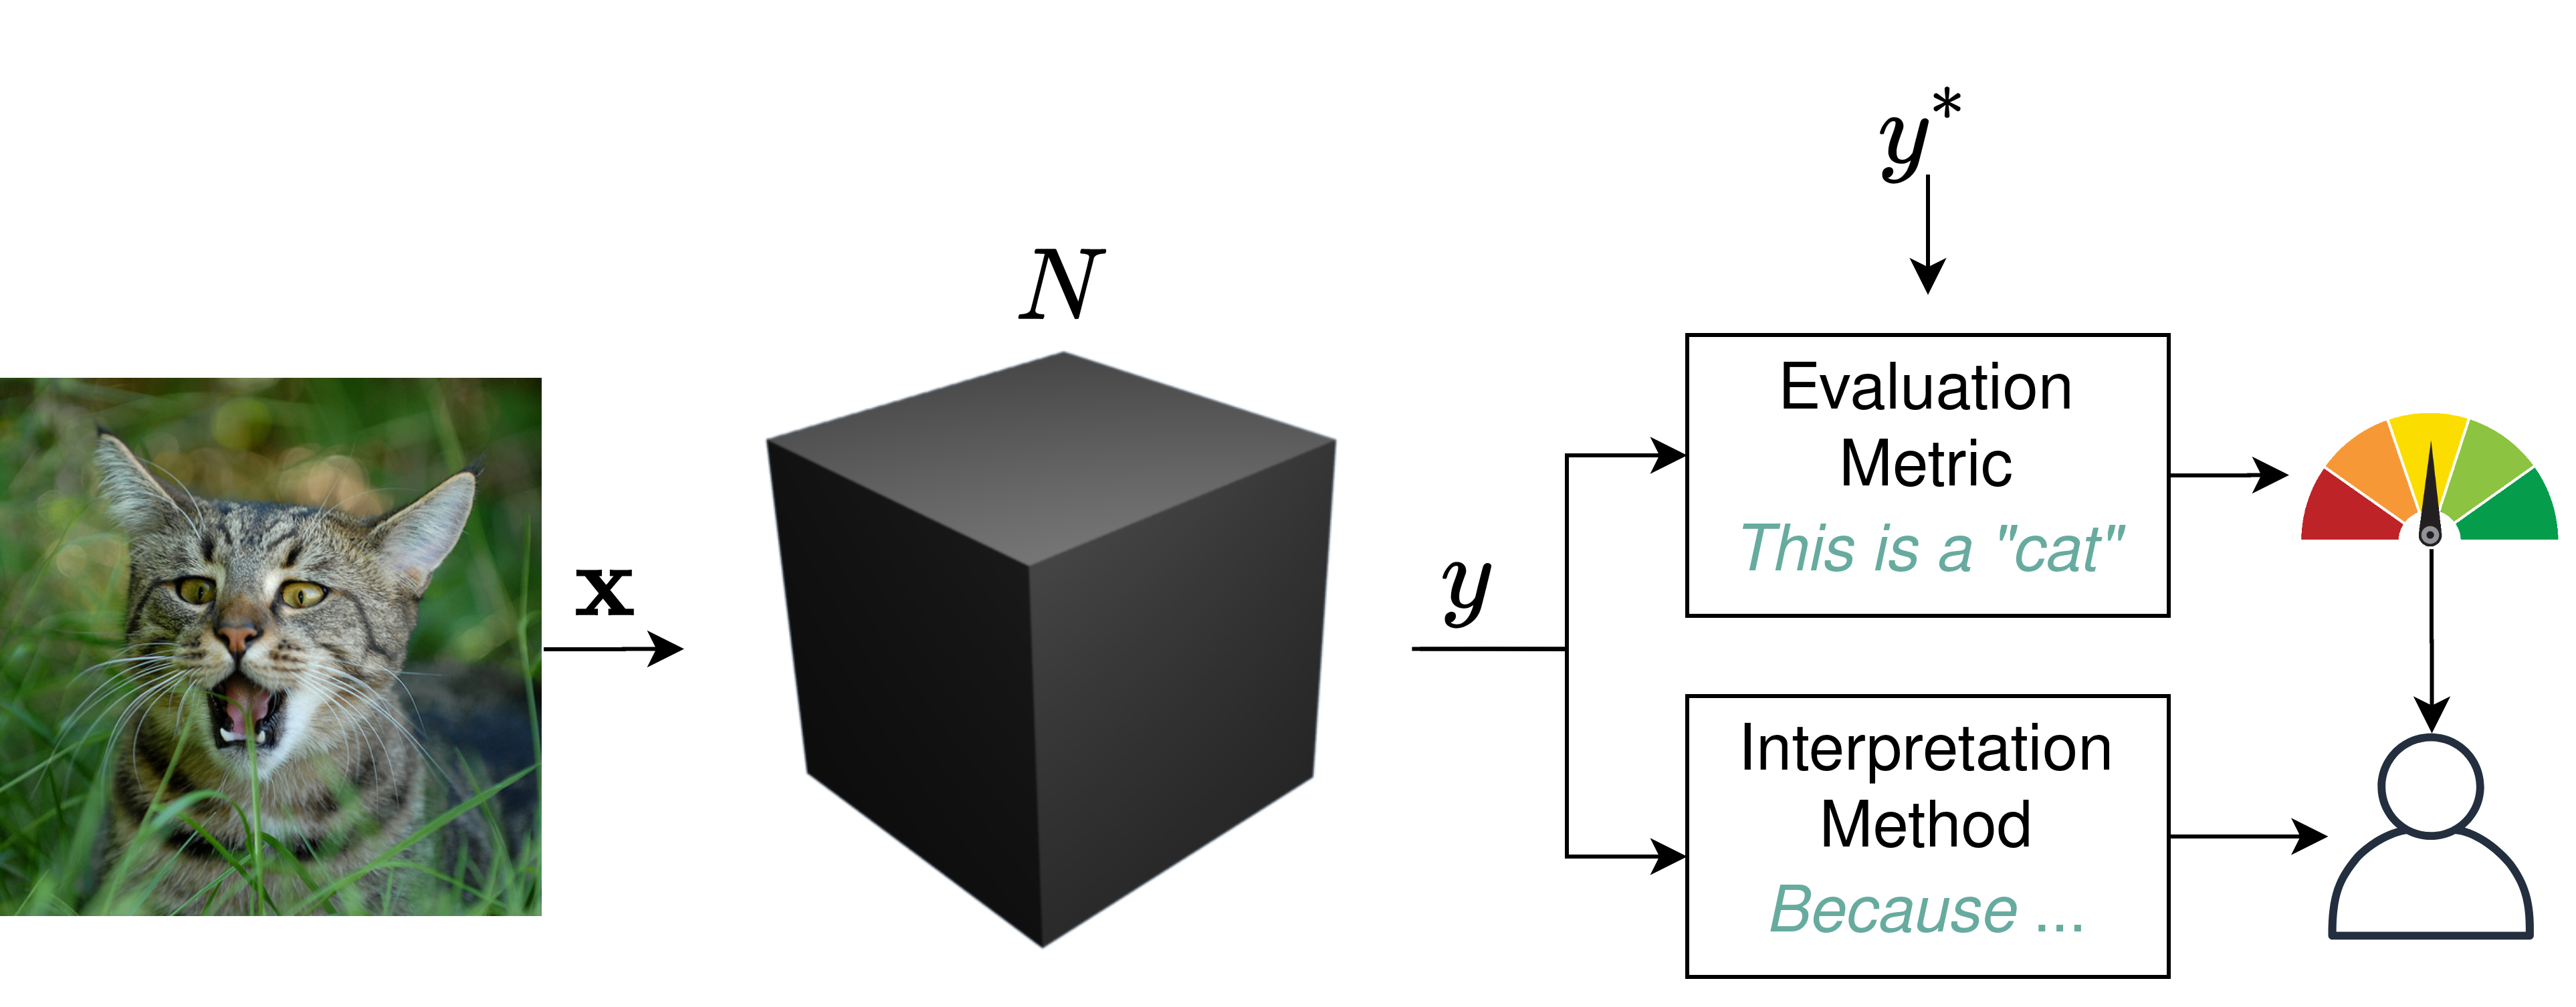
\includegraphics[width=\linewidth]{figures/bb_cat.png}
    \caption{Prediction pipeline using a machine learning model, depicted as a black box. Typically, evaluation metrics require the prediction $y$ and the ground truth label $y^*$ allowing for the assessmant of the model's accuracy. Additionally answering the question \textit{why}, i.e. making the model interpretable for a human, requires additional methods.}
    \label{fig:bb}
    \vspace{-0.3cm}
\end{figure}

Automated algorithms are already in use in critical areas, such as medicine, chemistry, the criminal justice system, the financial sector or the piloting of self-driving cars \cite{chouldechova2017fair, elshawi2019interpretability, whitmore2016mapping}. % med, med, chemistry
Thus, as machine learning models are moving out of the lab into the real-world, the inability of humans to understand these (black box) models seems even more problematic. Not knowing how a model makes predictions, and not being able to detect systematic biases in the model, prevents the vastly advancing technology of machine learning from being used in highly sensitive and safety-critical applications.  

Suppose a deep neural network predicts the risk for cancer from a mammogram, which is an image of breast tissue. A doctor would only use the algorithm if there is a way to validate that (1) the algorithm is accurate (which can be measured in terms of the predictive accuracy), and (2) if the model is also using the correct indications in the data for predicting the risk of cancer. (1) is the standard approach for validating the performance of machine learning models, but in this example, one can clearly see why predictive accuracy might not be enough in many areas. For approaching (2), i.e. uncovering \textit{why} a model predicts a low / high risk of cancer, the research field of explainable artificial intelligence (XAI) offers a fast growing number of methods. Some research even suggests to allow 'peeking inside the black box' of deep learning models \cite{adadi2018peeking}.  

%%%%%%%%%%%%%%%%%%
% In addition to this insecurity on the model level, it is likely that machine learning systems in deployment will be attacked. 

%%%%% iai
The threats of adversarial attacks on deployments of machine learning models has contributed to the field of XAI comprising topics of (1) \textit{model interpretations}, (2) \textit{adversarial attacks}, or manipulation methods and (3) the field of \textit{adversarial manipulations of model interpretations}. All these subfields have the common goal to make models more robust and safe for deployment. 
(1) refers to the development of techniques that can be used to understand and explain the decision making process of a machine learning model or even the development of models that are inherently interpretable. (2) is the field of detecting vulnerabilities in models that cause these models to be deceived by altered input. 
(3) is the main topic of this paper, i.e. how to fool interpretation methods in order to detect vulnerabilities and malfunctions in interpretation methods. 
%%%% 
Ideally, an interpretation or explanation method should indicate which features in the input to a model contribute to the prediction and also to what extent each feature contributes. This notion of extent is often called the \textit{importance} score of a feature. \autoref{fig:lrp_cat} shows such a feature importance map (\autoref{fig:lrp_cat_lrp}) produced by the interpretation method LRP \cite{bach2015pixel} applied to the neural network model Inception-v3 \cite{szegedy2016rethinking}. The input image is from the ImageNet dataset \cite{ILSVRC15}. The output of the interpretation method is projected onto the original image for better human readability. This importance map suggests that specific portions of the original cat image are important for the neural network make the high-confidence prediction (see..) of the category 'tiger cat'. 

\begin{figure}[ht]
    \centering
    \begin{subfigure}{0.32\linewidth}
      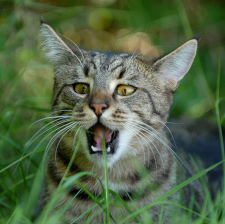
\includegraphics[width=\linewidth]{figures/cat.JPEG}
      \caption{Original.}
      \label{fig:lrp_cat_orig}
    \end{subfigure}
    \begin{subfigure}{0.32\linewidth}
      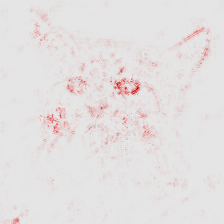
\includegraphics[width=\linewidth]{figures/lrp_cat_heatmap.png}
      \caption{Map.}
      \label{fig:lrp_cat_lrp}
    \end{subfigure}
    \begin{subfigure}{0.32\linewidth}
      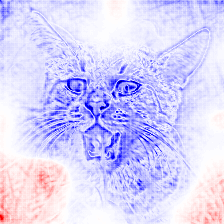
\includegraphics[width=\linewidth]{figures/foolignns/location fooling lrp/lrp_epoch6_no-7.png}
      \caption{Fooled Map.}
      \label{fig:lrp_cat_fooled_lrp}
    \end{subfigure}
    % \begin{subfigure}{0.8\linewidth}
    %     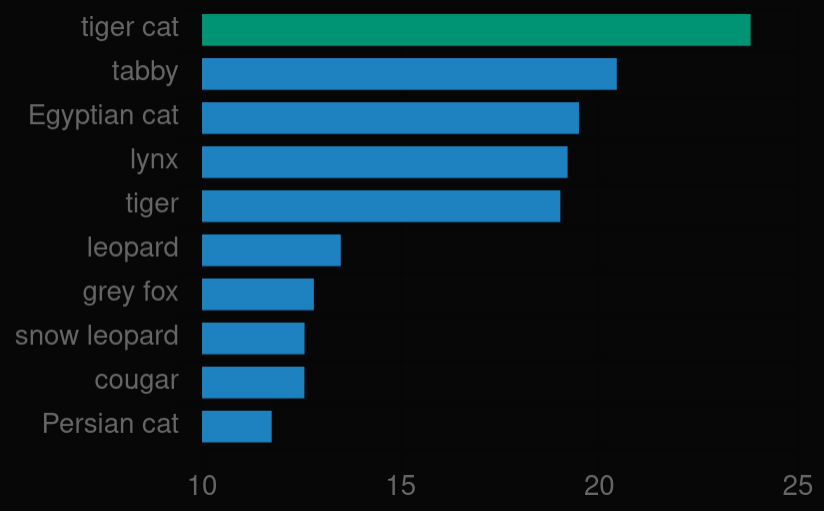
\includegraphics[width=\linewidth]{figures/cat_classification.png}
    %     \caption{Predictive accuracy.}
    %     \label{fig:cat_classification}
    % \end{subfigure}
    \caption{Visualization of the feature importance and fooled feature importance maps produced py the LRP interpreter applied to the image of a cat and an image classification model. The fooling method is the \textit{location} fooling from \cite{fooling_nn_interpreters}. Dark red here means a stronger significance of the feature.}\label{fig:lrp_cat}
    \vspace{-0.3cm}
\end{figure}

% https://towardsdatascience.com/interpretability-in-machine-learning-70c30694a05f 
% biases in ml models - boils down to data

% https://dl.acm.org/doi/pdf/10.1145/3387514.3405859?casa_token=lCc16GOTZsEAAAAA:gypLNU1o2Wwl3wt_b8stRbb0mgxEomX8PWprPeciNdkhVften3-5E01RM50e0W9NGQaGd4TrLOhA

While interpretation methods are already used for analysis of computer vision systems \cite{bach2015pixel, simonyan2013deep, zeiler2014visualizing}, text and sequence analysis \cite{ancona2017towards, arras2017relevant}, and deep learning in security \cite{evaluating_explanations_security}, there is still a lack in the the understanding of model interpretation methods. 
Recent work has shown, that humans are not able to benefit much from interpretation techniques: They cannot build better models and improve their own performance \cite{hase2020evaluating}, are not better at detecting false model decisions even in transparent models \cite{poursabzi2018manipulating}, and even data scientists over-trust and misuse model interpretation methods \cite{kaur2020interpreting}. 
Methodologically, it is unclear how the variety of proposed model interpretation methods are related and what common concepts can be used to evaluate and compare them. Many works are dedicated to establish a formal definition of what it means for a model to be interpretable, and how to select and evaluate methods for generating interpretations of machine learning models \cite{murdoch2019definitions, lipton2018mythos}. However, a growing number of researchers also focus on breaking these interpretation methods, similar to research on adversarial attacks on machine learning models, which is deeply fueled by the vast deployment of models in the real world \cite{fooling_nn_interpreters,ghorbani2019interpretation,dimanov2020you,dombrowski2019explanations,advlime_aies20, le2020remote, zhang2020interpretable, kuppa2020black, anders2020fairwashing, lakkaraju2020fool, kindermans2017reliability}.

% %%%%%%%%%%%%%%%%%%%%%%%%%%%%%%%%%%%%%%%%%%%%%%
% \subsection{Why is Interpretability Important?}
% \label{subsec:importance_of_interpretability}

% First, interpretability is helpful as it can help to build trust in a machine learning application. 
% % Suppose a neural network predicts the risk for cancer from a mammogram, which is an image of breast tissue. A doctor would only use the algorithm if there is a way to validate that (1) tha algorithm is accurate (which can be measured in terms of the predictive accuracy), and (2) if the model is also using the correct indications in the data for predicting the risk of cancer. (1) is the standard approach for validating the performance of machine learning models, but in this example, one can clearly see why predictive accuracy might not be enough. For approaching (2), i.e. uncovering \textit{why} a model predicts a low / high risk of cancer, a variety of interpretation methods are proposed.  
% % Ideally, an interpretation, or explanation method should indicate which pixels in the original image contribute to the prediction and also to what extent each pixel contributes. The extent to which each pixel contributes to a prediction is often called the \textit{importance} score of a feature. 

% The advantage of post-hoc interpretations is that they do not interfere with the training process of the model, and thus do not change the model. As the name says, post-hoc means that the techniques can be easily applied to an already trained model without much further computational overhead. 

% % https://thegradient.pub/interpretability-in-ml-a-broad-overview/ intro motvation
% % https://towardsdatascience.com/why-how-interpretable-ml-7288c5aa55e4 also

% High interpretability is desired as it can help to to uncover biases in the model. Suppose a machine learning model is to be deployed for the task of income prediction based on features such as age, race, gender, education and hours of work per week. The performance of the system would mainly be evaluated in terms oft the predictive accuracy and the fairness of the system. The former can be evaluated with metrics, such as accuracy on a held-out test set. For the latter, interpretability methods might be applied to observe which input features are used by the model to predict the income. 
% % TODO note here that tha data from adult_income do actually not allow for these features to be more important than others. 
% If the model uses sensitive features, such as sex and race as important features, it is systematically biased and thus unfair. 

%%%%%%%%%%%%%%%%%%%%%%%% Outline
\mypar{Outline. }\newline
This article examines a topic at the intersection of interpretable and adversarial machine learning research. 
The overview presented in this article examines the existing literature and contributions in the field of XAI focusing on methods to manipulate explanation methods. We try to offer a comprehensive taxonomy of these interpretation manipulation methods. 

This paper is structured as follows. \autoref{sec:interpretation_methods} introduces common interpretation methods for machine learning models, and offers a taxonomy of the variety of techniques and a brief outline of popular interpretation methods.
In \autoref{sec:manipulation_methods}, the main topic of this paper, namely manipulation methods for deceiving interpretation techniques, is outlined. A taxonomy of methods is proposed and possible evaluation criteria are listed. \autoref{sec:benchmarking} proposes approaches to benchmark the robustness of interpretation techniques and \autoref{sec:manipulations} provides a review of important studies in the field of manipulation methods. The implications of this research area on XAI are discussed in section \autoref{sec:discussion}.


%%%%%%%%%%%%%%%%%%%%%%%%%%%%%%%%%%%%%%%%%%%%%%%%%%%%%%%%%%%%%%%%%%%%%%%%%%%%%%%%%%%%%%%%%%%%%%%%%%%%%%%%
%%%%%%%%%%%%%%%%%%%%%%%%%%%%%%%%%%%%%%%%%%%%%%%%%%%%%%%%%%%%%%%%%%%%%%%%%%%%%%%%%%%%%%%%%%%%%%%%%%%%%%%%
% \section{Interpretation Methods}
\label{sec:interpretation_methods}

There exists a variety of definitions in the vastly expanding research field of XAI, and the concept of \textit{interpretability} still has no formal commonly used technical meaning \cite{lipton2018mythos}. To build on the common ground of existing research, this work follows the terminology of Lipton et al. \cite{lipton2018mythos} and Arrieta et al. \cite{arrieta2020explainable}.

Broadly, interpretabiity focuses on \textit{how} and \textit{why} a machine learning model makes predictions.
Simply put, interpretability is focused on getting some notion of an explanation for the decisions made by a machine learning model.

%%%%%%%%%%%%%%%%%%%%%%%%%%%%%%%%%%%%%%%%%%%%%%
\subsection{Terminology}
\label{subsec:interpretation_methods_terminology}
The authors of \cite{arrieta2020explainable} make a distinction between the related but different concepts of \textit{interpretability} and \textit{explainibility}. Lipton \cite{lipton2018mythos} further breaks down interpretability into \textit{transparency} and \textit{post-hoc} interpretability. The notion of \textit{explainibility} from \cite{arrieta2020explainable} can be related to Liptons's \textit{transparency}, while Lipton's \textit{post-hoc} interpretability is essentially \textit{interpretability} as defined by Arrieta et al. \cite{arrieta2020explainable}.

\mypar{Post-hoc Interpretability} refers to the the extent to which cause and effect can be observed in a model, which can be translated to uncovering \textit{why} a model made prediction $y$ to an input $\mathbf{x}$, or how input and output ralate. Consider the example of image classification from \autoref{fig:bb}. Here, interpretability would mean that if a cat is present in the image (the cause), the model classifies it to the category 'cat' (the effect). Now imagine we find that the model takes the green meadow in the image as evidence to predict 'cat', and not the cat itself. This would imply a lack of interpretability, as the model learns to assign features to the concept 'cat' other than those related to 'cat' in the correct sense. This toy example emphasizes a common problem in image classification: \cite{xiao2020noise} observe the over-reliance of models on image background, rather than on objects in the foreground. % Note that interpretabe AI cannot verify if the learned relationships between features and outputs is truly causal (tha meadow in tha image can be correlated to the image category, e.g. when most images depictiong a cat shows cats on green meadows. This is a correlation of features but not necessarily a causilaty in tha sense of 'meadow --> cat'. ) https://www.pnas.org/content/pnas/116/44/22071.full.pdf causal inference
% Simply put, interpretability is focused on getting some notion of an explanation for the decisions made by a machine learning model.

\mypar{Explainibility or Transparency} on the other hand spans methods to uncover \textit{how} a model makes predictions, meaning to observe the inner workings of a model and thus to literally explain what is happening in terms of understanding of the mechanisms by which a model works. Thus, tansparency refers to the model's inherent properties that can be known before the training process and that are helpful to understand the model.

\par\smallskip
While both concepts seem to be important for the general objective of explainable artificial intelligence, this paper focuses on post-hoc interpretability.
There are essentially two ways to achieve interpretability: (1) to use inherently interpretable models or (2) to post-process a model in a fashion that allows to yield insights. The former is known as the development of \textit{surrogate} models and more generally described as \textit{model-agnostic} methods. Option (2) is known as \textit{model-transparent} methods. 

\mypar{Local and Global Methods.} A further categorization can be made based on the scope of interpretations: \textit{Local} methods aim at providing interpretations that are true for a single data points and its neighbors. 
\textit{Global} methods aim at gaining interpretations that are valid for most data points in a class \cite{kim2018interpretability, nguyen2017plug, yosinski2015understanding}. The interpretation methods discussed within this paper mostly fall into the class of local explanation methods \cite{ribeiro2016should, lundberg2017unified, bach2015pixel}. % TODO add all?

\mypar{Feature Attribution Methods and Sample Attribution Methods. } Interpretation methods aim at making complex and inherently uninterpretable black box models interpretable by creating human readable visualizations. 
A frequently used type of explanation methods are \textit{feature attributions} mapping each input feature to a numeric score. This score should quantify the importance of the feature relative to the model output. The resulting attribution map is then visualized as a heatmap projected onto the input sample. This allows humans to interpret which input attributes are the most helpful for making tha final prediction. Sample attribution methods on the other hand interpret the model performance in terms of the importance of training examples from the dataset. 

We propose the following formal definition for interpretation method:\newline

\textbf{Definition 1: Interpretation Method.}

\setlength{\leftskip}{0.39cm}

  \noindent We consider a neural network $N: \mathbb{R}^d \to \mathbb{R}^k$. For the an arbitrary classification task, $N$ classifies an input sample $\mathbf{x}\in \mathbb{R}$ in $k$ categories where the prediction $f_N(\mathbf{x})=y \in \{1, ..., K\}$ is given by $y = arg max_i f_N(\mathbf{x})_i$.

  Given the neural network $N$, it's input vector $\mathbf{x} \in \mathbb{R}^d$ and the the neural networks prediction for input $\mathbf{x}$, $f_N(\mathbf{x})=y$, an interpretation method $\mathcal{I}$ determines why label $y$ has been chosen by $N$ for input $\mathbf{x}$. 
  The interpretation is given by an output vector $\mathbf{h_k} \in \mathbb{R}^d$ for a class $k$ where each entry $h_i$ is mostly a numeric value describing the relevance for the $i$-th input feature $x_i$ of $\mathbf{x}$ for the final score $f_N(\mathbf{x})$.

\setlength{\leftskip}{0pt}
\par\smallskip\vspace{-0.1cm}

As $\mathbf{h}$ has the same dimensions as the input $\mathbf{x}$ it can be mapped to the input, overlaying $\mathbf{x}$ as a heatmap, where the color value represents the importance of feature $x_i$ towards the prediction $f_N(\mathbf{x})$.
An example is given in \autoref{fig:lrp_cat_lrp}. Higher values, implying a stronger relative importance for making the prediction $f_N(\mathbf{x})$, are depicted in dark red. 

% A model-transparent interpretation method, in the following named interpreter $\mathcal{I}$, generates a heatmap
%  $$h_c^\mathcal{I}(\boldsymbol{\omega}) = \mathcal{I}(\mathbf{x}, c; \boldsymbol{\omega})$$
%   for a neural network with parameters $\boldsymbol{\omega}$ and class $c$. The heatmap is a vector $h_c^\mathcal{I}(\boldsymbol{\omega}) \in \mathbb{R}^d$, where the $j$-th value $h_{c, j}^\mathcal{I}(\boldsymbol{\omega})$ represents the importance score of the $j-th$ input feature $x_j$ for the final score of class $c$.

While all explanation methods try to obtain importance measures for the network prediction, they differ with respect to how these measures are obtained. \cite{evaluating_explanations_security} propose two major categories for interpretation strategies, namely \textit{black-box}, in the following named \textit{model-agnostic} methods and \textit{white-box}, or \textit{} interpretation methods. 
While black-box interpretations assume no knowledge about the underlying model, white-box methods only work by using the model parameters. 

This terminology of discriminating between black-box and white-box methods may not be confused with the nature of the underlying models: Models still remain of black-box nature even though a white-box method may contribute to making the decision making process of such a model more insightful. % The opposite ofblack-box-nessistransparency,i.e., the search for a direct understanding of the mechanism by which a model works [5] 


The following section details the two categories and will give examples of the state-of-the-art interpretation methods within each group. 

% \noindent\textbf{Black-box Methods.} Black-box interpretations assume no knowledge about the model thus treating it as a black-box. The underlying model is approximated by learning it's behavior with an interpretable model, e.g. a linear model. As the model itself does not need to be known for using such a model-agnostic approach, thy can be used in scenarios where the model itself is not directly accessible. A black-box interpretation offers the big advantage to be applicable to any model.


% \noindent\textbf{White-box Methods.} On the other side are white-box interpretations, where the model is known with all its parameters. Thus, the explanations can be directly computed by using the model instead of relying on an approximation of $f_N$ as within the black-box models. As within these white-box models, tha model parameters can be used for calculating the interpretations, these methods are also named gradient or saliency map based methods. 

\subsection{Model-agnostic methods.}
\label{subsec:bb_methods}

% https://proceedings.neurips.cc//paper/2020/file/2c29d89cc56cdb191c60db2f0bae796b-Paper.pdf p. 4 
Model-agnostic interpretations assume no knowledge about the model thus treating it as a black box. The underlying model is approximated by learning it's behavior with an interpretable model, e.g. a linear model. The interpretable model is also dubbed the 'surrogate' model. The common approach for learning the surrogate is to approximate the relationship between the input samples and the corresponding prediction by tho model.
As the model itself does not need to be known, these approaches can be used in scenarios where the model itself is not directly accessible. Model-agnostic interpretations are fairly popular and are used in a wide range of applications, ranging from finance and law to medicine and chemistry \cite{elshawi2019interpretability, whitmore2016mapping}. 

A black-box interpretation offers the great advantage of being applicable to any model and offers simplicity because the interpretation is embedded in the model. However, this option of gaining interpretability might be costly for users that already have a high performing model. For this reason, growing need for methods exists that can be applied without retraining or modifying the underlying model.
We will briefly describe two common model-agnostic approaches. Refer to the original papers for details.

\mypar{Local Interpretable Model-agnostic Explanations (LIME).}\newline
LIME \cite{ribeiro2016should} perturbs the input and observes how the predictions of a black box model change. For the task of image classification, LIME creates a set of perturbed instances by dividing the input image into interpretable components, which are technically contiguous superpixels, and runs each perturbed instance through the model to get the probability for how much the change in each superpixel influences the whole model prediction. 

\autoref{fig:lime_cat} shows an example of LIME applied to the neural network model Inception-v3 \cite{szegedy2016rethinking}. Input image from the ImageNet dataset \cite{ILSVRC15}. The superpixel in dog instances place is highlighted in green, which correctly indicates that this superpixel has a high influence on the prediction of the images correct class ('bernese mountain dog'). LIME also correctly indicates that the superpixel in the cat's place does not indicate the correct class label.

\begin{figure}[ht]
  \centering
  \begin{subfigure}{0.32\linewidth}
    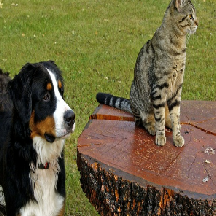
\includegraphics[width=\linewidth]{figures/lime_orig.png}
    \caption{Original}
    \label{fig:bird-a}
  \end{subfigure}
  \begin{subfigure}{0.32\linewidth}
    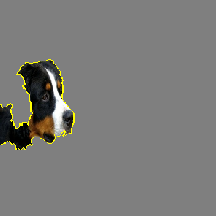
\includegraphics[width=\linewidth]{figures/lime_dog_mask.png}
    \caption{Mask.}
    \label{fig:bird-a}
  \end{subfigure}
  \begin{subfigure}{0.32\linewidth}
    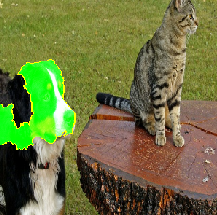
\includegraphics[width=\linewidth]{figures/lime_dog_map1.png}
    \caption{Saliency Map.}
    \label{fig:bird-a}
  \end{subfigure}
  \caption{Visualization of the output of the LIME interpreter applied to an image and image classification model.}\label{fig:lime_cat}
  \vspace{-0.3cm}
\end{figure}

% https://github.com/marcotcr/lime
% While the model may be very complex globally, it is easier to approximate it around the vicinity of a particular instance. While treating the model as a black box, we perturb the instance we want to explain and learn a sparse linear model around it, as an explanation. The figure below illustrates the intuition for this procedure. The model's decision function is represented by the blue/pink background, and is clearly nonlinear. The bright red cross is the instance being explained (let's call it X). We sample instances around X, and weight them according to their proximity to X (weight here is indicated by size). We then learn a linear model (dashed line) that approximates the model well in the vicinity of X, but not necessarily globally.


\mypar{SHapley Additive exPlanations (SHAP).} SHAP \cite{lundberg2017unified} builds on Shapley analysis, which is essentially about judging the importence of attibutes. The model is trained on a number of subsets of all available features, and the feature importance scores are calculated by evaluating the effects that the omissions of the specific features have on the model prediction. An example is shown in \autoref{fig:shap_dog}. Image regions highlighted in green are found to be important for predicting the correct label.

\begin{figure}[ht]
  \centering
  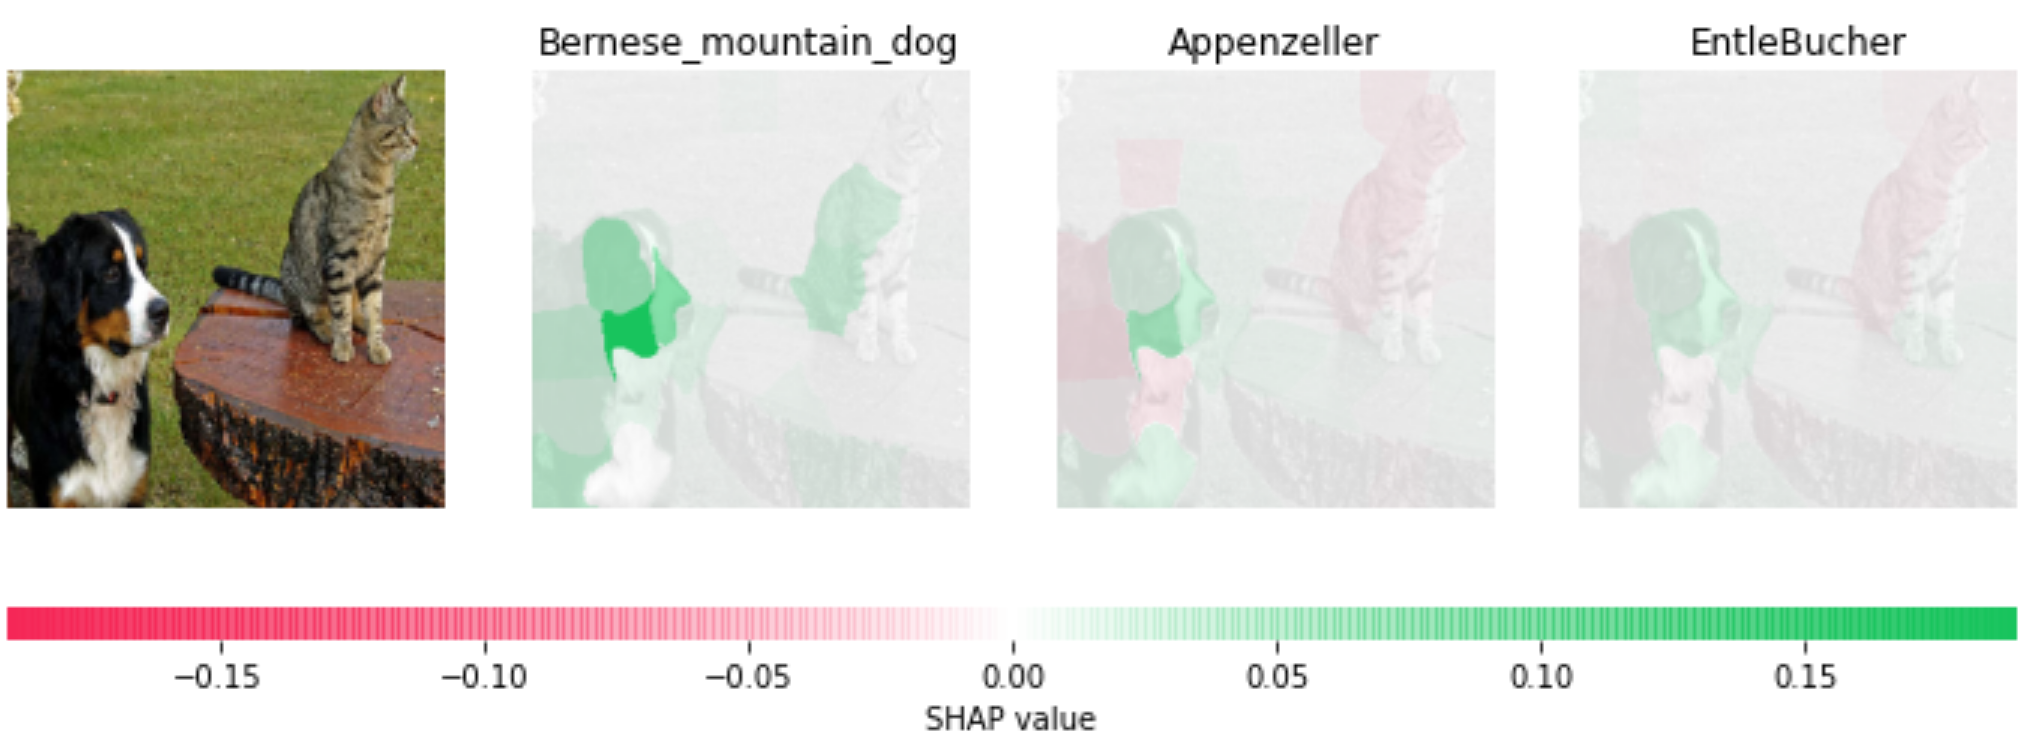
\includegraphics[width=\linewidth]{figures/cat_dog_shap.png}
  \caption{Visualization of the output of the SHAP interpreter applied to applied to an image and image classification model.}\label{fig:shap_dog}
  \vspace{-0.3cm}
\end{figure}


\subsection{Model-transparent methods.}
\label{subsec:wb_methods}

The other group of interpretations are model-transparent, or white-box methods, where the underlying model is known with all its parameters. Thus, the interpretation can be directly computed by using the model instead of relying on an approximation of $f_N$ as within the black-box methods. These methods typically rely on the relationship between an input sample, the underlying model's prediction and the associated activations of the models hidden layers. Methods within this group are for example propagation-based and gradient-based approaches. The former propagate back the model's prediction back through the model. The latter make use of the information provided by the gradients of the loss function, which contain sensitive information about the prediction and the features. Using the backpropagation method, features in the input can be highlighted based on the amount of gradient they receive. This shows their contribution to the final score. 
A few example methods within this group are listed below. 

\mypar{Layer-wise Relevance Propagation (LRP).} While many approaches in the group of model-transparent interpretations are designed only for image classification, or convolutional neural networks, this method \cite{bach2015pixel} is an exception. LRP propagates relevance values backwards through the network and decomposes the score of a predicted class backwards through the network. It relies on a Taylor series close to the prediction point rather than partial derivatives at the prediction point itself. An example for a feature map produced by LRP can be found in \autoref{fig:lrp_cat_lrp}.
%The output is a heatmap of relevance values, depicting for each feature how helpful or harmful the feature is for predicting the target class. 

\mypar{DeepLIFT} \cite{shrikumar2017learning} is an improved version of LRP, where a reference point in the input feature space is defined. Relevance scores are propagated proportionally to the changes of neuronal activations from the reference. % https://arxiv.org/pdf/1710.10547.pdf

\mypar{SmoothGrad (SG)} \cite{smilkov2017smoothgrad} avarages over interpretations of noisy copies of an input sample thus reducing noise by visually diffusing the interpretation. The noise is drawn from i.i.d. from a normal distribution. 

Methods developed for convolutional neural networks are for instace GradCAM \cite{selvaraju2017grad} or SimleGrad TODOcite. 
% \mypar{Gradient-weighted Class Activation Mapping (Grad-CAM)}
% Grad-CAM \cite{selvaraju2017grad} uses the gradients of any target concept, flowing into the final convolutional layer to produce a coarse localization map, highlighting the important regions in the image for predicting the concept.

% \mypar{SimpleGrad (SimpleG)}

% Please see the original publications for more detailed information. 
\section{Interpretation Methods}
\label{sec:interpretation_methods}

There exists a variety of definitions in the vastly expanding research field of XAI, and the concept of \textit{interpretability} still has no formal commonly used technical meaning \cite{lipton2018mythos}. To build on the common ground of existing research, this work follows the terminology of Lipton et al. \cite{lipton2018mythos} and Arrieta et al. \cite{arrieta2020explainable}.

Broadly, interpretabiity focuses on \textit{how} and \textit{why} a machine learning model makes predictions.
Simply put, interpretability is focused on getting some notion of an explanation in human understandable terms for the decisions made by a machine learning model.

%%%%%%%%%%%%%%%%%%%%%%%%%%%%%%%%%%%%%%%%%%%%%%
\subsection{Terminology}
\label{subsec:interpretation_methods_terminology}
The authors of \cite{arrieta2020explainable} make a distinction between the related but different concepts of \textit{interpretability} and \textit{explainibility}. Lipton \cite{lipton2018mythos} further breaks down interpretability into \textit{transparency} and \textit{post-hoc} interpretability. The notion of \textit{explainibility} from \cite{arrieta2020explainable} can be related to Liptons's \textit{transparency}, while Lipton's \textit{post-hoc} interpretability is essentially \textit{interpretability} as defined by Arrieta et al. \cite{arrieta2020explainable}.

\mypar{Post-hoc Interpretability} refers to the the extent to which cause and effect can be observed in a model, which can be translated to uncovering \textit{why} a model made prediction $y$ to an input $\mathbf{x}$, or how input and output ralate. Consider the example of image classification from \autoref{fig:bb}. Here, interpretability would mean that if a cat is present in the image (the cause), the model classifies it to the category 'cat' (the effect). Now imagine we find that the model takes the green meadow in the image as evidence to predict 'cat', and not the cat itself. This would imply a lack of interpretability, as the model learns to assign features to the concept 'cat' other than those related to 'cat' in the correct sense. This toy example emphasizes a common problem in image classification: \cite{xiao2020noise} observe the over-reliance of models on image background, rather than on objects in the foreground. % Note that interpretabe AI cannot verify if the learned relationships between features and outputs is truly causal (tha meadow in tha image can be correlated to the image category, e.g. when most images depictiong a cat shows cats on green meadows. This is a correlation of features but not necessarily a causilaty in tha sense of 'meadow --> cat'. ) https://www.pnas.org/content/pnas/116/44/22071.full.pdf causal inference
% Simply put, interpretability is focused on getting some notion of an explanation for the decisions made by a machine learning model.

\mypar{Explainibility or Transparency} on the other hand spans methods to uncover \textit{how} a model makes predictions, meaning to observe the inner workings of a model and thus to literally explain what is happening in terms of understanding of the mechanisms by which a model works. Thus, tansparency refers to the model's inherent properties that can be known before the training process and that are helpful to understand the model.

\par\smallskip\vspace*{-0.3cm}
While both concepts seem to be important for the general objective of explainable artificial intelligence, this paper focuses on post-hoc interpretability.
There are essentially two ways to achieve interpretability: (1) to use inherently interpretable models or (2) to post-process a model in a fashion that allows to yield insights. The former is known as the development of \textit{surrogate} models and more generally described as \textit{model-agnostic} methods. Option (2) is known as \textit{model-transparent} methods. 

\mypar{Local and Global Methods.} A further categorization can be made based on the scope of interpretations: \textit{Local} methods aim at providing interpretations that are true for a single data points and its neighbors. 
\textit{Global} methods aim at gaining interpretations that are valid for most data points in a class \cite{kim2018interpretability, nguyen2017plug, yosinski2015understanding}. The interpretation methods discussed within this paper mostly fall into the class of local explanation methods \cite{ribeiro2016should, lundberg2017unified, bach2015pixel}. % TODO add all?

\mypar{Feature Attribution Methods and Sample Attribution Methods. } Interpretation methods aim at making complex and inherently uninterpretable black box models interpretable by creating human readable visualizations. 
A frequently used type of explanation methods are \textit{feature attributions} mapping each input feature to a numeric score. This score should quantify the importance of the feature relative to the model output. The resulting attribution map is then visualized as a heatmap projected onto the input sample. This allows humans to interpret which input attributes are the most helpful for making tha final prediction. Sample attribution methods on the other hand interpret the model performance in terms of the importance of training examples from the dataset. 

We adhere to the following formal definition for interpretation method:\newline

\textbf{Definition 1: Interpretation Method.}

\setlength{\leftskip}{0.39cm}

  \noindent We consider a neural network $N: \mathbb{R}^d \to \mathbb{R}^k$. For the an arbitrary classification task, $N$ classifies an input sample $\mathbf{x}\in \mathbb{R}$ in $k$ categories where the prediction $f_N(\mathbf{x})=y \in \{1, ..., K\}$ is given by $y = arg max_i f_N(\mathbf{x})_i$.

  Given the neural network $N$, it's input vector $\mathbf{x} \in \mathbb{R}^d$ and the the neural networks prediction for input $\mathbf{x}$, $f_N(\mathbf{x})=y$, an interpretation method $\mathcal{I}$ determines why label $y$ has been chosen by $N$ for input $\mathbf{x}$. 
  The interpretation is given by an output vector $\mathbf{h_k} \in \mathbb{R}^d$ for a class $k$ where each entry $h_i$ is mostly a numeric value describing the relevance for the $i$-th input feature $x_i$ of $\mathbf{x}$ for the final score $f_N(\mathbf{x})$.

\setlength{\leftskip}{0pt}
\par\smallskip\vspace{-0.1cm}

As $\mathbf{h}$ has the same dimensions as the input $\mathbf{x}$ it can be mapped to the input, overlaying $\mathbf{x}$ as a heatmap, where the color value represents the importance of feature $x_i$ towards the prediction $f_N(\mathbf{x})$.
An example is given in \autoref{fig:lrp_cat_lrp}. Higher values, implying a stronger relative importance for making the prediction $f_N(\mathbf{x})$, are depicted in dark red. 

While all explanation methods try to obtain importance measures for the network prediction, they differ with respect to how these measures are obtained. \cite{evaluating_explanations_security} propose two major categories for interpretation strategies, namely \textit{black-box}, in the following named \textit{model-agnostic} methods and \textit{white-box}, or \textit{model-transparent} interpretation methods. 
While black-box interpretations assume no knowledge about the underlying model, white-box methods only work by using the model parameters. 

This terminology of discriminating between black-box and white-box methods may not be confused with the nature of the underlying models: Models still remain of black-box nature even though a white-box method may contribute to making the decision making process of such a model more insightful.

The following section details the two categories and gives examples of commonly used interpretation methods within each group. 

\subsection{Model-agnostic methods.}
\label{subsec:bb_methods}

% https://proceedings.neurips.cc//paper/2020/file/2c29d89cc56cdb191c60db2f0bae796b-Paper.pdf p. 4 
Model-agnostic interpretations assume no knowledge about the model thus treating it as a black box. The underlying model is approximated by learning it's behavior with an interpretable model, e.g. a linear model. The interpretable model is also dubbed the 'surrogate' model. The common approach for learning the surrogate is to approximate the relationship between the input samples and the corresponding prediction by tho model.
As the model itself does not need to be known, these approaches can be used in scenarios where the model itself is not directly accessible. Model-agnostic interpretations are fairly popular and are used in a wide range of applications, ranging from finance and law to medicine and chemistry \cite{elshawi2019interpretability, whitmore2016mapping}. 

A black-box interpretation offers the great advantage of being applicable to any model and offers simplicity because the interpretation is embedded in the model. However, this option of gaining interpretability might be costly for users that already have a high performing model. For this reason, growing need for methods exists that can be applied without retraining or modifying the underlying model.
We will briefly describe two common model-agnostic approaches. Please refer to the original papers for details.

\mypar{Local Interpretable Model-agnostic Explanations (LIME).}\newline
LIME \cite{ribeiro2016should} perturbs the input and observes how the predictions of a black box model change. For the task of image classification, LIME creates a set of perturbed instances by dividing the input image into interpretable components, which are technically contiguous superpixels, and runs each perturbed instance through the model to get the probability for how much the change in each superpixel influences the whole model prediction. 

\autoref{fig:lime_cat} shows an example of LIME applied to the neural network model Inception-v3 \cite{szegedy2016rethinking}. Input image from the ImageNet dataset \cite{ILSVRC15}. The superpixel in dog instances place is highlighted in green, which correctly indicates that this superpixel has a high influence on the prediction of the images correct class ('bernese mountain dog'). LIME also correctly indicates that the superpixel in the cat's place does not indicate the correct class label.

\begin{figure}[ht]
  \centering
  \begin{subfigure}{0.32\linewidth}
    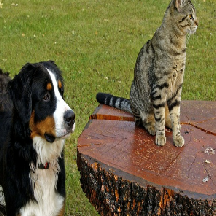
\includegraphics[width=\linewidth]{figures/lime_orig.png}
    \caption{Original}
    \label{fig:bird-a}
  \end{subfigure}
  \begin{subfigure}{0.32\linewidth}
    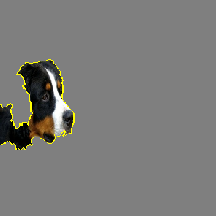
\includegraphics[width=\linewidth]{figures/lime_dog_mask.png}
    \caption{Mask.}
    \label{fig:bird-a}
  \end{subfigure}
  \begin{subfigure}{0.32\linewidth}
    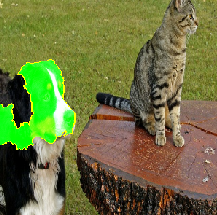
\includegraphics[width=\linewidth]{figures/lime_dog_map1.png}
    \caption{Saliency Map.}
    \label{fig:bird-a}
  \end{subfigure}
  \caption{Visualization of the output of the LIME interpreter applied to an image and image classification model.}\label{fig:lime_cat}
  \vspace{-0.3cm}
\end{figure}

% https://github.com/marcotcr/lime
% While the model may be very complex globally, it is easier to approximate it around the vicinity of a particular instance. While treating the model as a black box, we perturb the instance we want to explain and learn a sparse linear model around it, as an explanation. The figure below illustrates the intuition for this procedure. The model's decision function is represented by the blue/pink background, and is clearly nonlinear. The bright red cross is the instance being explained (let's call it X). We sample instances around X, and weight them according to their proximity to X (weight here is indicated by size). We then learn a linear model (dashed line) that approximates the model well in the vicinity of X, but not necessarily globally.

\mypar{SHapley Additive exPlanations (SHAP).} SHAP \cite{lundberg2017unified} builds on Shapley analysis, which is essentially about judging the importence of attibutes. The model is trained on a number of subsets of all available features, and the feature importance scores are calculated by evaluating the effects that the omissions of the specific features have on the model prediction. An example is shown in \autoref{fig:shap_dog}. Image regions highlighted in green are found to be important for predicting the correct label.

\begin{figure}[ht]
  \centering
  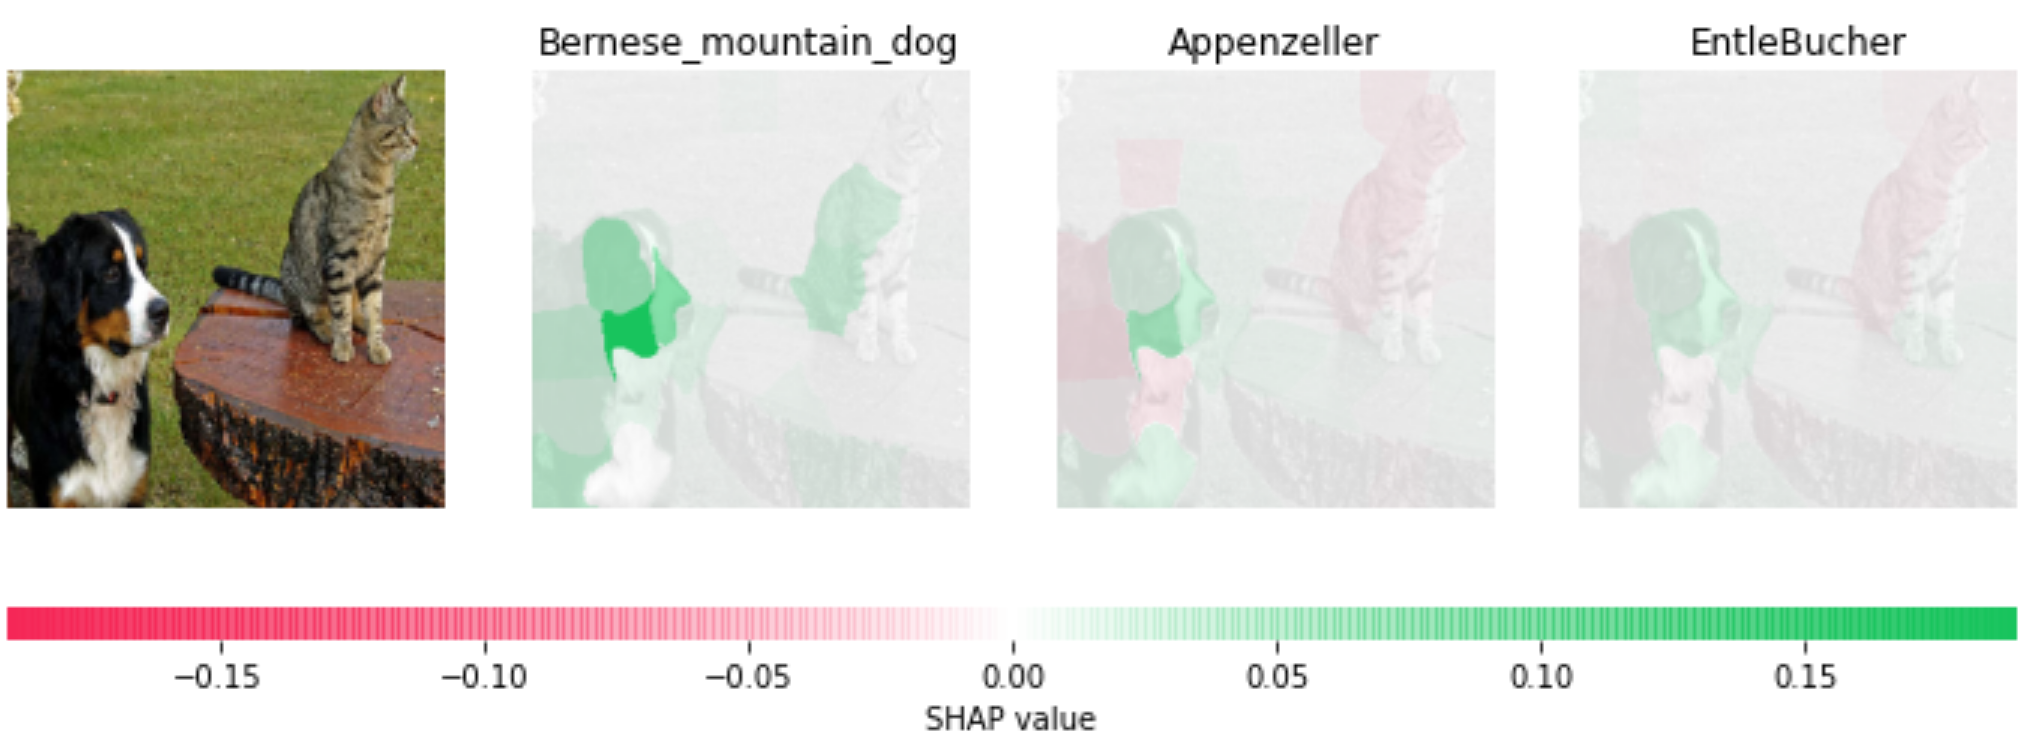
\includegraphics[width=\linewidth]{figures/cat_dog_shap.png}
  \caption{Visualization of the output of the SHAP interpreter applied to applied to an image and image classification model.}\label{fig:shap_dog}
  \vspace{-0.3cm}
\end{figure}


\subsection{Model-transparent methods.}
\label{subsec:wb_methods}

The other group of interpretations are model-transparent, or white-box methods, where the underlying model is known with all its parameters. Thus, the interpretation can be directly computed by using the model instead of relying on an approximation of $f_N$ as within the black-box methods. These methods typically rely on the relationship between an input sample, the underlying model's prediction and the associated activations of the models hidden layers. Methods within this group are for example propagation-based and gradient-based approaches. The former propagate back the model's prediction back through the model. The latter make use of the information provided by the gradients of the loss function, which contain sensitive information about the prediction and the features. Using the backpropagation method, features in the input can be highlighted based on the amount of gradient they receive. This shows their contribution to the final score. 
A few example methods within this group are listed below. 

\mypar{Layer-wise Relevance Propagation (LRP).} While many approaches in the group of model-transparent interpretations are designed only for image classification, or convolutional neural networks, this method \cite{bach2015pixel} is an exception. LRP propagates relevance values backwards through the network and decomposes the score of a predicted class backwards through the network. It relies on a Taylor series close to the prediction point rather than partial derivatives at the prediction point itself. An example for a feature map produced by LRP can be found in \autoref{fig:lrp_cat_lrp}.
%The output is a heatmap of relevance values, depicting for each feature how helpful or harmful the feature is for predicting the target class. 

\mypar{DeepLIFT} \cite{shrikumar2017learning} is an improved version of LRP, where a reference point in the input feature space is defined. Relevance scores are propagated proportionally to the changes of neuronal activations from the reference. % https://arxiv.org/pdf/1710.10547.pdf

\mypar{SmoothGrad (SG)} \cite{smilkov2017smoothgrad} avarages over interpretations of noisy copies of an input sample thus reducing noise by visually diffusing the interpretation. The noise is drawn from i.i.d. from a normal distribution. 

Methods developed for convolutional neural networks are for instance GradCAM \cite{selvaraju2017grad} or SimpleGrad. % TODO cite  


%%%%%%%%%%%%%%%%%%%%%%%%%%%%%%%%%%%%%%%%%%%%%%%%%%%%%%%%%%%%%%%%%%%%%%%%%%%%%%%%%%%%%%%%%%%%%%%%%%%%%%%%
%%%%%%%%%%%%%%%%%%%%%%%%%%%%%%%%%%%%%%%%%%%%%%%%%%%%%%%%%%%%%%%%%%%%%%%%%%%%%%%%%%%%%%%%%%%%%%%%%%%%%%%%
% \section{Manipulation Methods}
\label{sec:manipulation_methods}

As outlined in \autoref{sec:interpretation_methods}, there are a variety of explanation methods readily available as frameworks and open source implementations. However, there is still little analysis on the robustness and reliability of such methods. 
While it is already common practice to test machine learning models against adversarial attacks in a number of domains \cite{gao2019universal, kereliuk2015deep}, the same is not yet the standard for interpretation methods. We argue that interpretation techniques should not be used in critical applications without basic testing of interpretation techniques against adversarial settings.

\subsection{Adversarial Setting}
\label{subsec:adversarial_setting}
\mypar{Adversarial Attacks on Models. }
Adversarial examples, as first introduced by \cite{szegedy_intriguing}, are clever manipulations of an input by an adversary which aims at causing misclassification and fooling of applications. They are mostly used to fool or attack machine learning models. We formally define adversarial attacks by the following properties: 
\par\smallskip
\textbf{Definition 2: Model Manipulation Method}
\begin{enumerate}
    \item[1.] \textit{Impercpetibility of Perturbation}: The adversal example is similar to original data, i.e. the norm of the added perturbation $\delta$ to an input sample $\mathbf{x}$ thus must be small, i.e. $$\norm{\mathbf{x}+\delta} = \norm{(\mathbf{x}+\delta)-\mathbf{x}}_{\inf} \leq \epsilon$$
    \item[2.] \textit{Prediction dissimilarity}: The prediction of the model is significantly different to the prediction on the non-adversarial example: $$f_N(\mathbf{x}+\delta) \approx f_N(\mathbf{x})$$
\end{enumerate}
Note, that within adversarial foolings of models, the perturbation is mostly applied to the input data, and not to the model itself.

% TODO cite
Evidence from many studios shows that deep learning models can be easily tricked by adversarial examples. 
Albeit there are not yet as many studies, there also exists evidence that many interpretation methods are also fragile with respect to small changes to input data \cite{adebayo2018sanity, samek2019explainable, alvarez2018towards} as well as to the model itself \cite{fooling_nn_interpreters, dimanov2020you}. This fooling of interpretation methods is outlined below. 

\mypar{Adversarial Attacks on Model Interpreters. } 
Contrary to adversarial attacks on machine learning models, the focus of this paper is on the attacks on interpretation techniques without changing the prediction of the model. 
An adversarial attack on a model interpretation is in the following also called a \textit{manipulation} method. 
The goal is to apply perturbations to either an input sample or the model to change the output of an interpretation technique while leaving the model prediction unchanged. The last condition is important because adversarial interpreter manipulations aim to fool the interpretation method and essentially not the model itself. 
Fooling the model would only disclose the vulnerability of the model but would not allow to gain insight into the stability of the interpretation method. 
Again, the problem can be formally defined as:

% A manipulation method refers to a method influencing an interpretation method $\mathcal{I}$ to yield a wrong interpretation. This influence on the interpretation method is also called \textit{fooling} or an \textit{attack}. 
\par\smallskip
\textbf{Definition 3: Interpretation Manipulation Method.}

\setlength{\leftskip}{0.39cm}
% as it is the goal to disclose the vulnerability of the explanation method and not the vulnerability of the model.
\noindent A manipulation method $\mathcal{F}$ is defined as a method for altering the output of an explanation method $\mathcal{I}$ while leaving the model performance of the neural network $N$ roughly unchanged. 
As manipulations can be applied on the input or the model level (see \autoref{subsubsec:manipulation_levels}), $\mathbf{x}+\delta$ denotes a perturbed input sample regarding the input level manipulation, while $N+\delta$ denotes a model with altered parameters, referring to the model level manipulation.

A manipulation method is successful in fooling an interpreter, if the following properties hold: 
\begin{enumerate}
    % TODO for all i, as in http://lcfi.ac.uk/media/uploads/files/DimanovBhattJamnikWeller_YouShouldntTrustMe.pdf 
    \item[1.] \textit{Prediction similarity}: The model prediction stays approximately the same, i.e. $$f_N(\mathbf{x}+\delta) \approx f_N(\mathbf{x}) \text{, or } f_{N+\delta}(\mathbf{x}) \approx f_N(\mathbf{x})$$
    % \item[2.] \textit{Interpretation dissimilarity}: The explanation map $h(\mathbf{x}+\delta)$ is significantly different to the explanation map resulting from non adversarial models or inputs $h(\mathbf{x})$, i.e. $h(\mathbf{x}+\delta)$ or $$\argmax_{\delta} = \mathcal{D}(\mathcal{I}(x_i, \boldsymbol{\omega}), \mathcal{I}(x_i+\delta, \boldsymbol{\omega})$$
    \item[2.] \textit{Imperceptibility of Perturbation}: In case the attack is in the input domain of the model, the perturbation of input samples must be imperceptible by humans. According to \cite{dombrowski2019explanations}, the norm of the added perturbation $\delta$ to an input sample $\mathbf{x}$ thus must be small, i.e. $$\norm{\mathbf{x}+\delta} = \norm{(\mathbf{x}+\delta)-\mathbf{x}}_{\inf} \leq \epsilon$$ % https://arxiv.org/pdf/1710.10547.pdf 
\end{enumerate}
\setlength{\leftskip}{0cm}

These measures are to be seen as comparison between a baseline model $N$ and a model that is applied an the adversarial setting (i.e. either $N$ is not changed but applied to adversarially altered data $x+\delta$, or $N$ is adversarially trained thus becoming $N+\delta$). 
Interpretation manipulation methods differ with respect to the definition of the fooling of the interpretation method. 
Some methods aim to make the interpreter give wrong interpretations\cite{fooling_nn_interpreters}. 
In this case, the following additional property must hold: 
\begin{enumerate}
   \item[3.] \textit{Interpretation dissimilarity}: The explanation map $h(\mathbf{x}+\delta)$ is significantly different to the explanation map resulting from non adversarial models or inputs $h(\mathbf{x})$, i.e. $h(\mathbf{x}+\delta)$ or $$\argmax_{\delta} = \mathcal{D}(\mathcal{I}(x_i, \boldsymbol{\omega}), \mathcal{I}(x_i+\delta, \boldsymbol{\omega}))$$ where $\mathcal{D}(\cdot)$ is a distance measure. 
\end{enumerate}

Others introduce a systematic bias into tho model while fooling the interpretation method in the sense that the interpretation does not change between the original model and the adversarial model. 
Here, it must hold that property 3. takes the minimal argument.
% TODO add image for this. 

\cite{dimanov2020you} extend these properties to include the so called \textit{model similarity}. This measure extends the \textit{prediction accuracy} to span the accuracy difference in between the baseline model and the new model, and also the mismatch of data points where the predictions of both models differ. 

After formally defining what successfully fooling an interpretation method means, we want to provide intuition in \autoref{fig:lrp_cat}. The interpretation method produces an interpretation, here in form of a saliency map projected onto the original image. If a successful manipulation is applied, the resulting saliency map of the same interpreter should be different to the original map. This effect is clearly visible, as \autoref{fig:lrp_cat_lrp} is visually significantly different to the map produced by the same interpretation method but applied to an adversarial model (see \autoref{fig:lrp_cat_fooled_lrp}). 

%%%%%%%%%%%%%%%%%%%%%%%%%
\subsection{Taxonomy of Interpretation Manipulation Methods}
\label{subsec:taxonomy_manipulations}
There are two important categories of Manipulation Methods that aim at attacking model interpretation methods. The first category is based on the level these manipulations operate on, i.e. input space level or model / paramater level. 
The second categorization is based on the target of the manipulations. While untargeted manipulations are mostly random perturbations, targeted manipulations aim to perturb the interpretation of specific input features. 

%%%%%%%%%%
\subsubsection{Manipulation Levels}
\label{subsubsec:manipulation_levels}
\par\smallskip
\noindent 

\par\smallskip
\noindent\textbf{Adversarial Input Manipulation.} The general approach is to perturb or alter input data while observing the effect of this perturbation on the model prediction. This concept is visualized in \autoref{fig:input_manipulation}. 
As found in \cite{dombrowski2019explanations}, visually-imperceptible perturbations of an input image can make explanations worse for the same model and interpreter. 

\begin{figure}[ht]
    \centering
    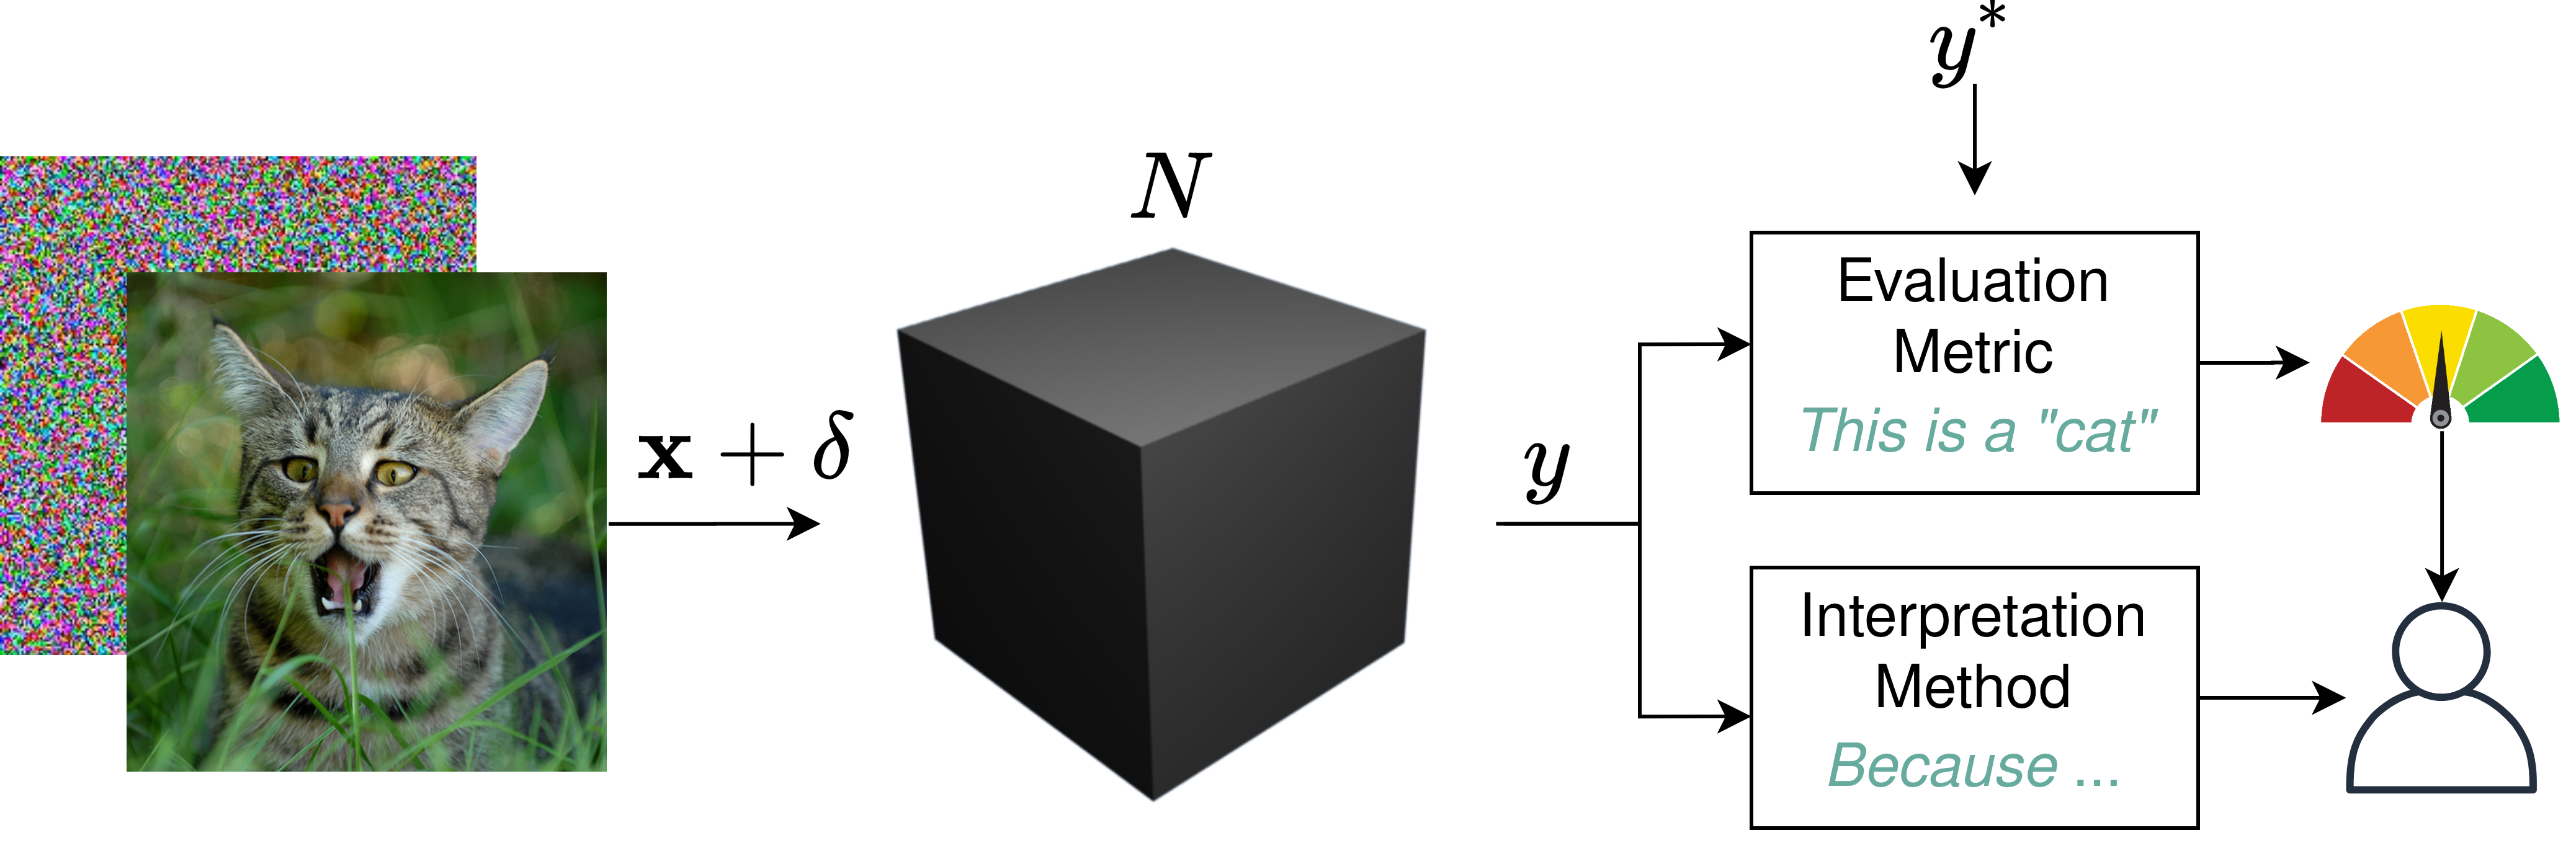
\includegraphics[width=\linewidth]{figures/input_manipulations.png}
    \caption{Depiction of an adversarial input manipulation. The model is fine-tuned with altered input samples, which are indicated by $\mathbf{x}+\delta$.}
    \label{fig:input_manipulation}
    \vspace{-0.3cm}
\end{figure}

\par\smallskip
\noindent\textbf{Adversarial Model Manipulation.} 
Contrary to input manipulations, model manipulations do not operate on the input space but rather on the model parameter space itself. 
As first introduced by Heo et al. \cite{fooling_nn_interpreters} in 2019, this line of research is comparably new. 
Adversarial model manipulations for fooling the interpreter are obtained by fine-tuning the model on the same data but with an adapted objective function. \cite{fooling_nn_interpreters} propose the adapted loss function for the task of image classification of $$ \mathcal{L} = \mathcal{L}_{CE}(\mathcal{D};\omega) + \lambda \cdot \mathcal{L}(\mathcal{D};\omega; \omega_0) $$ where $\mathcal{L}_{CE}$ is the standard cross-entropy classification loss. 
Adversarial model manipulation is depicted in \autoref{fig:input_manipulation} where the altered model is indicated by $N+\delta$.

\begin{figure}[ht]
    \centering
    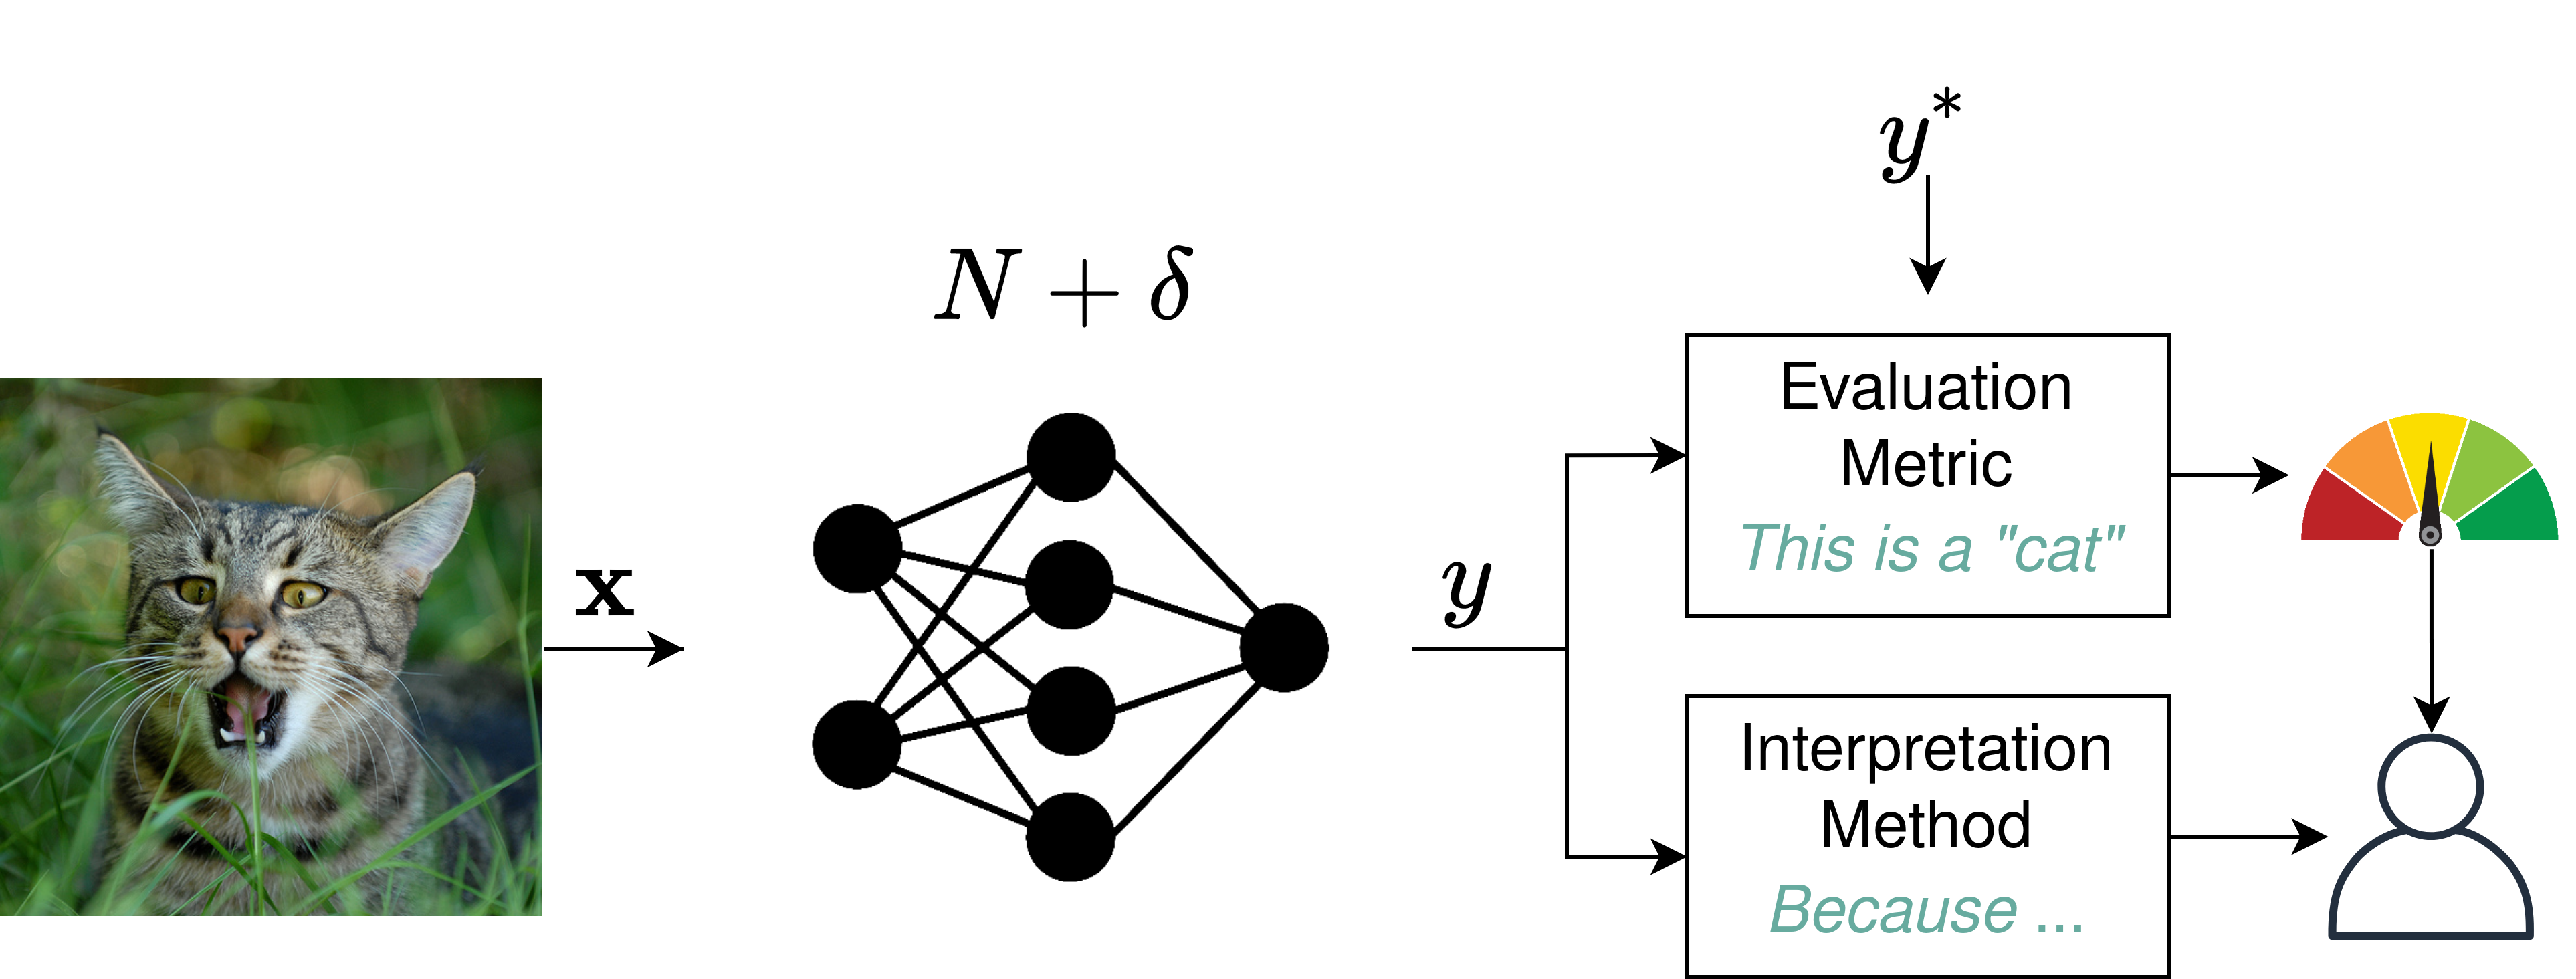
\includegraphics[width=\linewidth]{figures/model_manipulations.png}
    \caption{Depiction of an adversarial model manipulation. The model is fine-tuned with the same distribution of input data and a fooling loss, thus yielding the biased model $N+\delta$.}
    \label{fig:input_manipulation}
    \vspace{-0.3cm}
\end{figure}

%%%%%%%%%%
\subsubsection{Manipulation Targets}
\label{subsubsec:manipulation_targets}

\par\smallskip
\noindent
In addition to the categorization of manipulation methods based on the manipulation level, the methods can further be categorized based on the target of their perturbation. The first possibility is \textit{untargeted} perturbation, the second is \textit{targeted} perturbation. Both these styles can be applied on either model and input level. 

\mypar{Untargeted Manipulations.} 
The majority of manipulations is untargeted, meaning that the applied perturbations are mostly random and not designed to change the prediction for a specific portion of an input sample. 

\mypar{Targeted Manipulations.} 
On the contrary, targeted manipulations aim at specifically changing the explanation of certain features of an input instance \cite{fooling_nn_interpreters}, and sometimes even changing the interpretation of specific classes \cite{simonyan2013deep}. Such a specific feature might be an object in the input image in the context of image classification. \cite{fooling_nn_interpreters} for instance introduce a fooling scheme in which the interpretations of the target classes elephant and school bus are swapped. 
Manipulations on the level of the model are mostly targeted, as the explanation methods are being fooled by adapting the model parameters. 

% Model manipulations pose a much higher threat for deploying the models: If a model itself is changed to explicitly, systemactically fool an explanation method, the bias of the model is internal and much harder to reveal than just a different sort of input into the model. 

%%%%%%%%%%%%%%%%%%%%%%%%% 
\subsection{Evaluation Criteria}
\label{subsec:eval_criteria_manipulations}
Besides the necessary properties of a successful interpretation manipulation method, other evaluation criteria are important to access the success of a fooling method as well as to enable the comparison between different fooling methods. These criteria are informally defined in the following.

\mypar{Effectiveness.} The manipulation scheme is inexpensive to conduct. Input manipulations are by definition inexpensive, as the perturbation can be applied to single input samples. Model manipulations are more expensive as they require tho model parameters to be adapted. However, an adversarial model can be obtained by fine-tuning the model with an adapted objective function. This fine-tuning also has the advantage that the model is adapted to include a systematic bias and can thus be applied to fool explanation methods without further adapting the model or input samples after the fine-tuning step. Furthermore, this systematic bias is hidden in the model, and is hard to uncover. Input manipulations can only fool the model when the inputs are always manipulated. 

\mypar{Transferability.} The manipulation does not only fool one type of interpretation method, but it's effect transfers to other interpretation techniques. 
% This property is naturally given for the class of model manipulations


\mypar{Generalisation.} Generalization of an attack refers to the transfer of fooling to other test samples. This is noteworthy since a manipulation method might only perturb the decision boundary locally around the training points, i.e. only influencing training instances and their neighbors. However, it is desired that the explanations of unseen samples are affected as well. Furthermore, not only unseen samples intarpretations, but also samples that are far away in the feature space should be affected. 
Otherwise, the perturbation is only local around the training points, thus the perturbation does not generalize. 
% On the contrary, model manipulations are non-local perturbations, meaning that they do not merely perturb an input sample
% but rather effect all samples in the way that the model itself is changed. 
% TODO iid ood?
% The  generalisation  of  the  attack  to  testpoints  is  noteworthy  since  we  might  expect  that  the  deci-sion boundary would be perturbed locally around the train-ing points to affect only their explanations, without signifi-cant change for test points, especially if far away in featurespace (see Appendix for more)

\par\smallskip
As outlined in section \autoref{sec:manipulation_methods}, there exists a plethora of interpretation methods differing in the assumption about the model character and also with respect to how interpretations are obtained. Thus, reliable evaluation methods are required allowing for a choice of an appropriate and robust interpretation method. Ultimately, the accordance to these evaluations should naturally allow for choosing an appropriate and robust intarpretation method.  
Evaluations of the quality of an explanation method are separated into qualitative and quantitative evaluations. 

\mypar{Qualitative Evaluation.} 
Inspection and random sampling are commonly used techniques to obtain an intuition about the effect of manipulations. 
As interpretations are attributed to input features, the resulting relevance values $l$ can be easily mapped to the input vector $\mathbf{x}$. Visual inspection of these evaluations for specific samples is informative, but does not allow for general statistics and validation of manipulation effects. Thus, quantitative evaluations are required. 
\cite{adebayo2018sanity} consider two kinds of visualizing saliency maps: 
\begin{itemize}
    \item \textbf{Absolute Value (ABS).} Saliency maps visualized this way show only the absolute values of the normalizem maps.
    \item \textbf{Diverging. } The diverging visualization indicates positive and negative importance in different colors. 
\end{itemize}

\mypar{Quantitative Evaluation.} 
As the goal of interpreter manipulations is to fool an interpreter, thus altering the output of in interpreter, it is straightforward to compare interpretations and data samples before and after perturbation \cite{ghorbani2019interpretation}.

As interpreter manipulations shall alter the output of an interpretation methods while keeping the prediction of a model unchanged, the following metrics 

\begin{itemize}
    \item \textbf{Fooling Success Rate (FSR).} \cite{fooling_nn_interpreters} introduce the concept of the Fooling Success Rate (FSR). The FSR captures the relationship between the model's predictive accuracy and the correctness of the interpretation averaged over multiple test samples. The 'correctness' of the interpretation is the difference between the original interpretation methods output and the output of the same interpretation method when applied to either an adversarial input sample or adversarial model. 
    The FSR counts samples for the model's prediction did not change but for which the interpretation method's output changed as a successfully fooled example. Thus, the higher the FSR, the the more often the fooling is successful in fooling the interpretation method. 
    \item \textbf{Area Over Prediction Curve (AOPC). } AOPC \cite{samek2016evaluating} is a principled way of quantitatively evaluating that the interpretations found by interpretation methods are valid, i.e. based on the features that the model truly uses for making the predicton. \cite{fooling_nn_interpreters} use this measure to ensure that their adversarial model training does not fool the model (i.e. the predictive accuracy of the model is unchanged), but does fool the interpretation method.
\end{itemize}

As the goal of interpreter manipulations is to fool an interpreter, thus altering the output of in interpreter, it is straightforward to compare interpretations and data samples before and after perturbation \cite{ghorbani2019interpretation}.
There are metrics that are applied to identify changes in salient features for any task:
\begin{itemize}
    \item \textbf{Spearman's rank order correlation.} As interpretation methods rank the features based on their importance, the rank correlation \cite{spearman1961proof} is a natural meusure for comparing interpretations. 
    \item \textbf{Intersection of the top-$k$ features.} For some tasks, only the top-$k$ features are relevant, such that a comparison between these top-$k$ features is insightful. 
\end{itemize}

Contrary, the following metrics are used only in computer vision tasks. They have been used in literature to quantify similarities between natural images and remove duplicates. Therefore, they are used in XAI research to compare the changes between saliency maps before and after manipulation for computer vision tasks.
\begin{itemize}
    \item \textbf{Structural Similarity Index (SSIM).} SSIM values are relative similarity measure in the range $\left[0, 1\right]$, where larger values indicate higher similarity.
    \item \textbf{Pearson Correlation Coefficien (PCC).} PCC is also a relative similarity measure returning values in the range $\left[0, 1\right]$. Larger values indicate higher similarity.
    \item \textbf{Pearson Correlation of the Histogram of Gradients\newline (HOG). } Used by \cite{adebayo2018sanity} to indicate the intensity of change between two images. 
    \item \textbf{Mean Squared Error (MSE).} As an absolute error measure, values close to zero indicate high similarity. 
\end{itemize}

\noindent Note that these are only examples without demand for completeness. For further information see \cite{adebayo2018sanity}.
Normalizing these measures to yield values in $\left[0, 1\right]$ with a sum of one is good practice. 
Note that defining similarities that are similar to human vision is still an active area of research. 
\section{Manipulation Methods}
\label{sec:manipulation_methods}

As outlined in \autoref{sec:interpretation_methods}, there are a variety of explanation methods readily available as frameworks and open source implementations. However, there is still little analysis on the robustness and reliability of such methods. 
While it is already common practice to test machine learning models against adversarial attacks in a number of domains \cite{gao2019universal, kereliuk2015deep}, the same is not yet the standard for interpretation methods. We argue that interpretation techniques should not be used in critical applications without basic testing of interpretation techniques against adversarial settings.

\subsection{Adversarial Setting}
\label{subsec:adversarial_setting}
\mypar{Adversarial Attacks on Models. }
Adversarial examples, as first introduced by \cite{szegedy_intriguing}, are clever manipulations of an input by an adversary which aims at causing misclassification and fooling of applications. They are mostly used to fool or attack machine learning models. We formally define adversarial attacks by the following properties: 
\par\smallskip
\textbf{Definition 2: Model Manipulation Method}
\begin{enumerate}
    \item[1.] \textit{Impercpetibility of Perturbation}: The adversal example is similar to original data, i.e. the norm of the added perturbation $\delta$ to an input sample $\mathbf{x}$ thus must be small, i.e. $$\norm{\mathbf{x}+\delta} = \norm{(\mathbf{x}+\delta)-\mathbf{x}}_{\inf} \leq \epsilon$$
    \item[2.] \textit{Prediction dissimilarity}: The prediction of the model is significantly different to the prediction on the non-adversarial example: $$f_N(\mathbf{x}+\delta) \approx f_N(\mathbf{x})$$
\end{enumerate}
Note, that within adversarial foolings of models, the perturbation is mostly applied to the input data, and not to the model itself.

% TODO cite
Evidence from many studios shows that deep learning models can be easily tricked by adversarial examples. 
Albeit there are not yet as many studies, there also exists evidence that many interpretation methods are also fragile with respect to small changes to input data \cite{adebayo2018sanity, samek2019explainable, alvarez2018towards} as well as to the model itself \cite{fooling_nn_interpreters, dimanov2020you}. This fooling of interpretation methods is outlined below. 

\mypar{Adversarial Attacks on Model Interpreters. } 
Contrary to adversarial attacks on machine learning models, the focus of this paper is on the attacks on interpretation techniques without changing the prediction of the model. 
An adversarial attack on a model interpretation is in the following also called a \textit{manipulation} method. 
The goal is to apply perturbations to either an input sample or the model to change the output of an interpretation technique while leaving the model prediction unchanged. The last condition is important because adversarial interpreter manipulations aim to fool the interpretation method and essentially not the model itself. 
Fooling the model would only disclose the vulnerability of the model but would not allow to gain insight into the stability of the interpretation method. 
Again, the problem can be formally defined as:

% A manipulation method refers to a method influencing an interpretation method $\mathcal{I}$ to yield a wrong interpretation. This influence on the interpretation method is also called \textit{fooling} or an \textit{attack}. 
\par\smallskip
\textbf{Definition 3: Interpretation Manipulation Method.}

\setlength{\leftskip}{0.39cm}
% as it is the goal to disclose the vulnerability of the explanation method and not the vulnerability of the model.
\noindent A manipulation method $\mathcal{F}$ is defined as a method for altering the output of an explanation method $\mathcal{I}$ while leaving the model performance of the neural network $N$ roughly unchanged. 
As manipulations can be applied on the input or the model level (see \autoref{subsubsec:manipulation_levels}), $\mathbf{x}+\delta$ denotes a perturbed input sample regarding the input level manipulation, while $N+\delta$ denotes a model with altered parameters, referring to the model level manipulation.

A manipulation method is successful in fooling an interpreter, if the following properties hold: 
\begin{enumerate}
    % TODO for all i, as in http://lcfi.ac.uk/media/uploads/files/DimanovBhattJamnikWeller_YouShouldntTrustMe.pdf 
    \item[1.] \textit{Prediction similarity}: The model prediction stays approximately the same, i.e. $$f_N(\mathbf{x}+\delta) \approx f_N(\mathbf{x}) \text{, or } f_{N+\delta}(\mathbf{x}) \approx f_N(\mathbf{x})$$
    % \item[2.] \textit{Interpretation dissimilarity}: The explanation map $h(\mathbf{x}+\delta)$ is significantly different to the explanation map resulting from non adversarial models or inputs $h(\mathbf{x})$, i.e. $h(\mathbf{x}+\delta)$ or $$\argmax_{\delta} = \mathcal{D}(\mathcal{I}(x_i, \boldsymbol{\omega}), \mathcal{I}(x_i+\delta, \boldsymbol{\omega})$$
    \item[2.] \textit{Imperceptibility of Perturbation}: In case the attack is in the input domain of the model, the perturbation of input samples must be imperceptible by humans. According to \cite{dombrowski2019explanations}, the norm of the added perturbation $\delta$ to an input sample $\mathbf{x}$ thus must be small, i.e. $$\norm{\mathbf{x}+\delta} = \norm{(\mathbf{x}+\delta)-\mathbf{x}}_{\inf} \leq \epsilon$$ % https://arxiv.org/pdf/1710.10547.pdf 
\end{enumerate}
\setlength{\leftskip}{0cm}

These measures are to be seen as comparison between a baseline model $N$ and a model that is applied an the adversarial setting (i.e. either $N$ is not changed but applied to adversarially altered data $x+\delta$, or $N$ is adversarially trained thus becoming $N+\delta$). 
Interpretation manipulation methods differ with respect to the definition of the fooling of the interpretation method. 
Some methods aim to make the interpreter give wrong interpretations\cite{fooling_nn_interpreters}. 
In this case, the following additional property must hold: 
\begin{enumerate}
   \item[3.] \textit{Interpretation dissimilarity}: The explanation map $h(\mathbf{x}+\delta)$ is significantly different to the explanation map resulting from non adversarial models or inputs $h(\mathbf{x})$, i.e. $h(\mathbf{x}+\delta)$ or $$\argmax_{\delta} = \mathcal{D}(\mathcal{I}(x_i, \boldsymbol{\omega}), \mathcal{I}(x_i+\delta, \boldsymbol{\omega}))$$ where $\mathcal{D}(\cdot)$ is a distance measure. 
\end{enumerate}

Others introduce a systematic bias into tho model while fooling the interpretation method in the sense that the interpretation does not change between the original model and the adversarial model. 
Here, it must hold that property 3. takes the minimal argument.
% TODO add image for this. 

\cite{dimanov2020you} extend these properties to include the so called \textit{model similarity}. This measure extends the \textit{prediction accuracy} to span the accuracy difference in between the baseline model and the new model, and also the mismatch of data points where the predictions of both models differ. 

After formally defining what successfully fooling an interpretation method means, we want to provide intuition in \autoref{fig:lrp_cat}. The interpretation method produces an interpretation, here in form of a saliency map projected onto the original image. If a successful manipulation is applied, the resulting saliency map of the same interpreter should be different to the original map. This effect is clearly visible, as \autoref{fig:lrp_cat_lrp} is visually significantly different to the map produced by the same interpretation method but applied to an adversarial model (see \autoref{fig:lrp_cat_fooled_lrp}). 

%%%%%%%%%%%%%%%%%%%%%%%%%
\subsection{Taxonomy of Interpretation Manipulation Methods}
\label{subsec:taxonomy_manipulations}
There are two important categories of Manipulation Methods that aim at attacking model interpretation methods. The first category is based on the level these manipulations operate on, i.e. input space level or model / paramater level. 
The second categorization is based on the target of the manipulations. While untargeted manipulations are mostly random perturbations, targeted manipulations aim to perturb the interpretation of specific input features. 

%%%%%%%%%%
\subsubsection{Manipulation Levels}
\label{subsubsec:manipulation_levels}
\par\smallskip
\noindent 

\par\smallskip
\noindent\textbf{Adversarial Input Manipulation.} The general approach is to perturb or alter input data while observing the effect of this perturbation on the model prediction. This concept is visualized in \autoref{fig:input_manipulation}. 
As found in \cite{dombrowski2019explanations}, visually-imperceptible perturbations of an input image can make explanations worse for the same model and interpreter. 

\begin{figure}[ht]
    \centering
    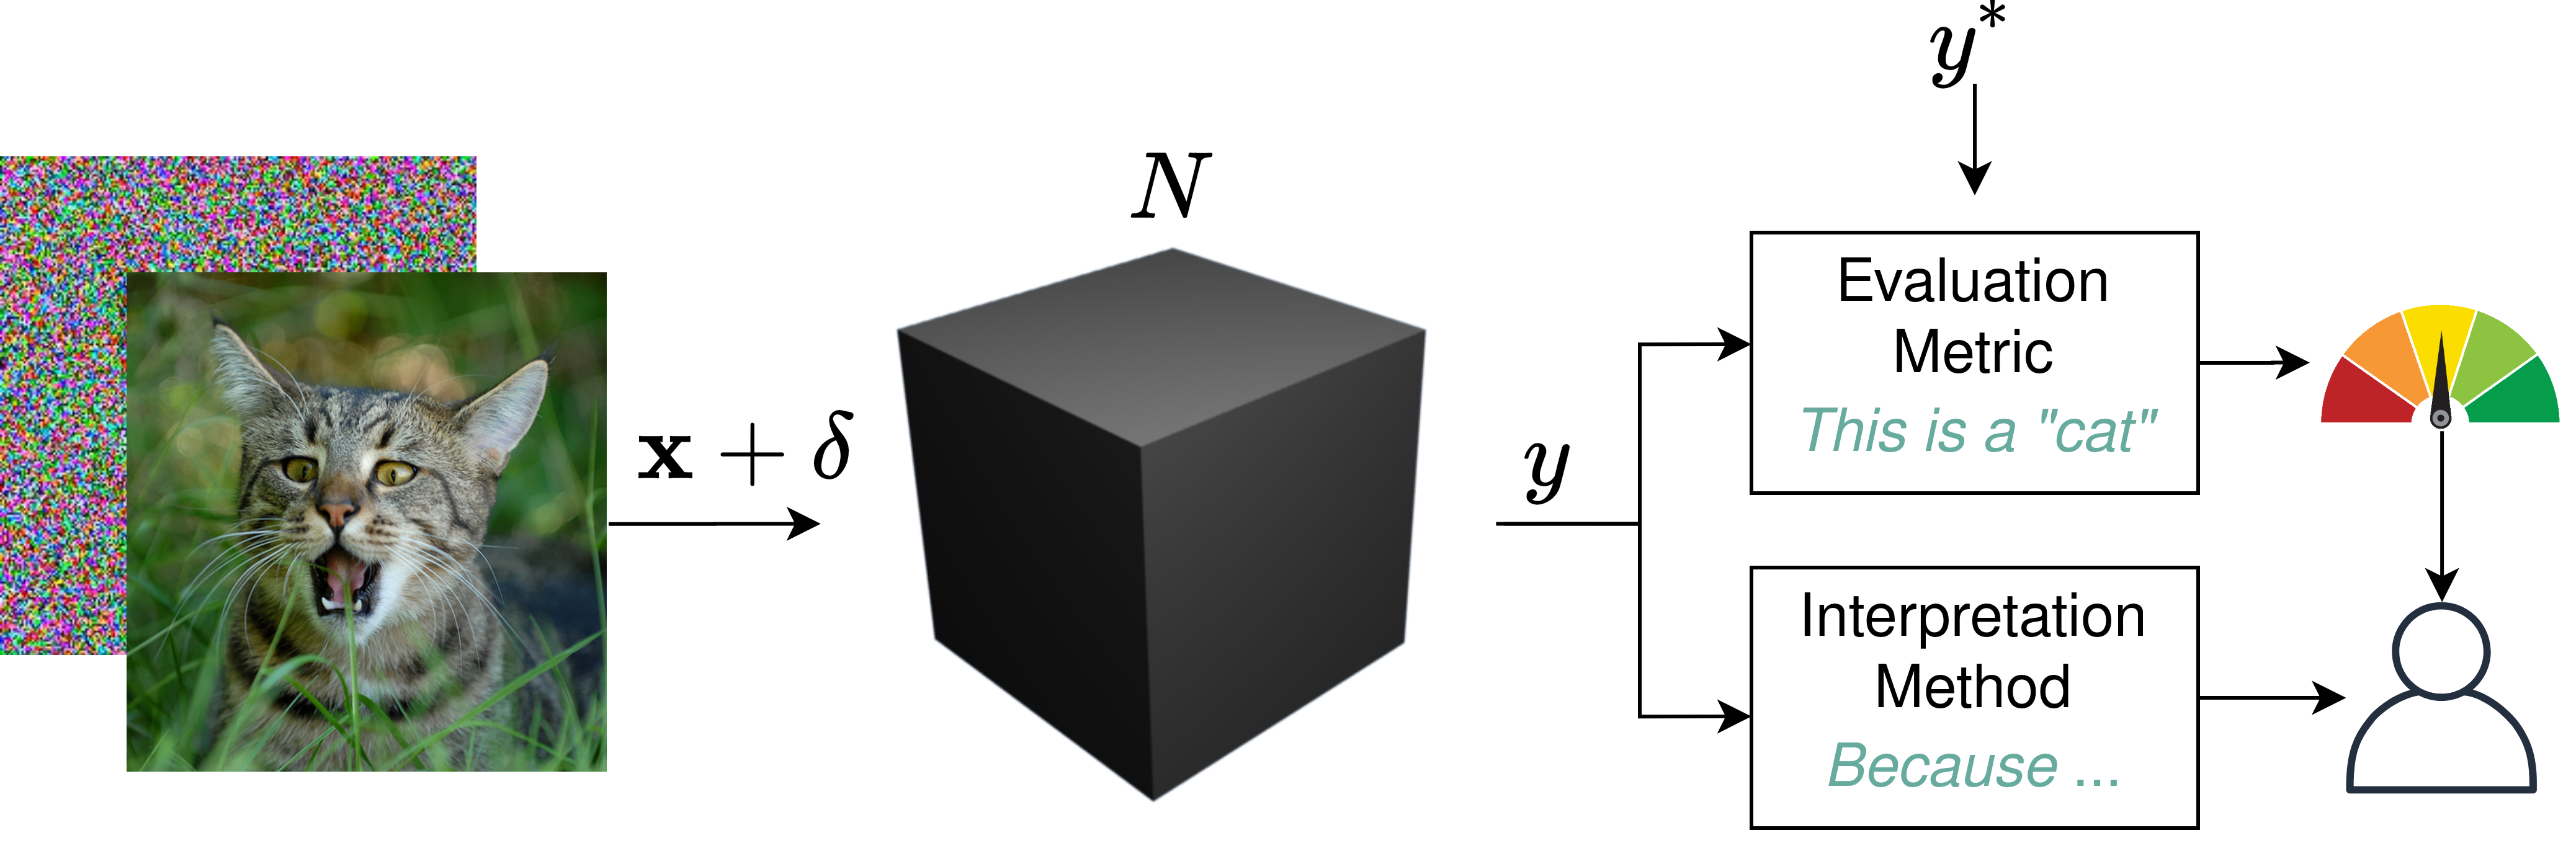
\includegraphics[width=\linewidth]{figures/input_manipulations.png}
    \caption{Depiction of an adversarial input manipulation. The model is fine-tuned with altered input samples, which are indicated by $\mathbf{x}+\delta$.}
    \label{fig:input_manipulation}
    \vspace{-0.3cm}
\end{figure}

\par\smallskip
\noindent\textbf{Adversarial Model Manipulation.} 
Contrary to input manipulations, model manipulations do not operate on the input space but rather on the model parameter space itself. 
As first introduced by Heo et al. \cite{fooling_nn_interpreters} in 2019, this line of research is comparably new. 
Adversarial model manipulations for fooling the interpreter are obtained by fine-tuning the model on the same data but with an adapted objective function. \cite{fooling_nn_interpreters} propose the adapted loss function for the task of image classification of $$ \mathcal{L} = \mathcal{L}_{CE}(\mathcal{D};\omega) + \lambda \cdot \mathcal{L}(\mathcal{D};\omega; \omega_0) $$ where $\mathcal{L}_{CE}$ is the standard cross-entropy classification loss. 
Adversarial model mbibliography
\begin{figure}[ht]
    \centering
    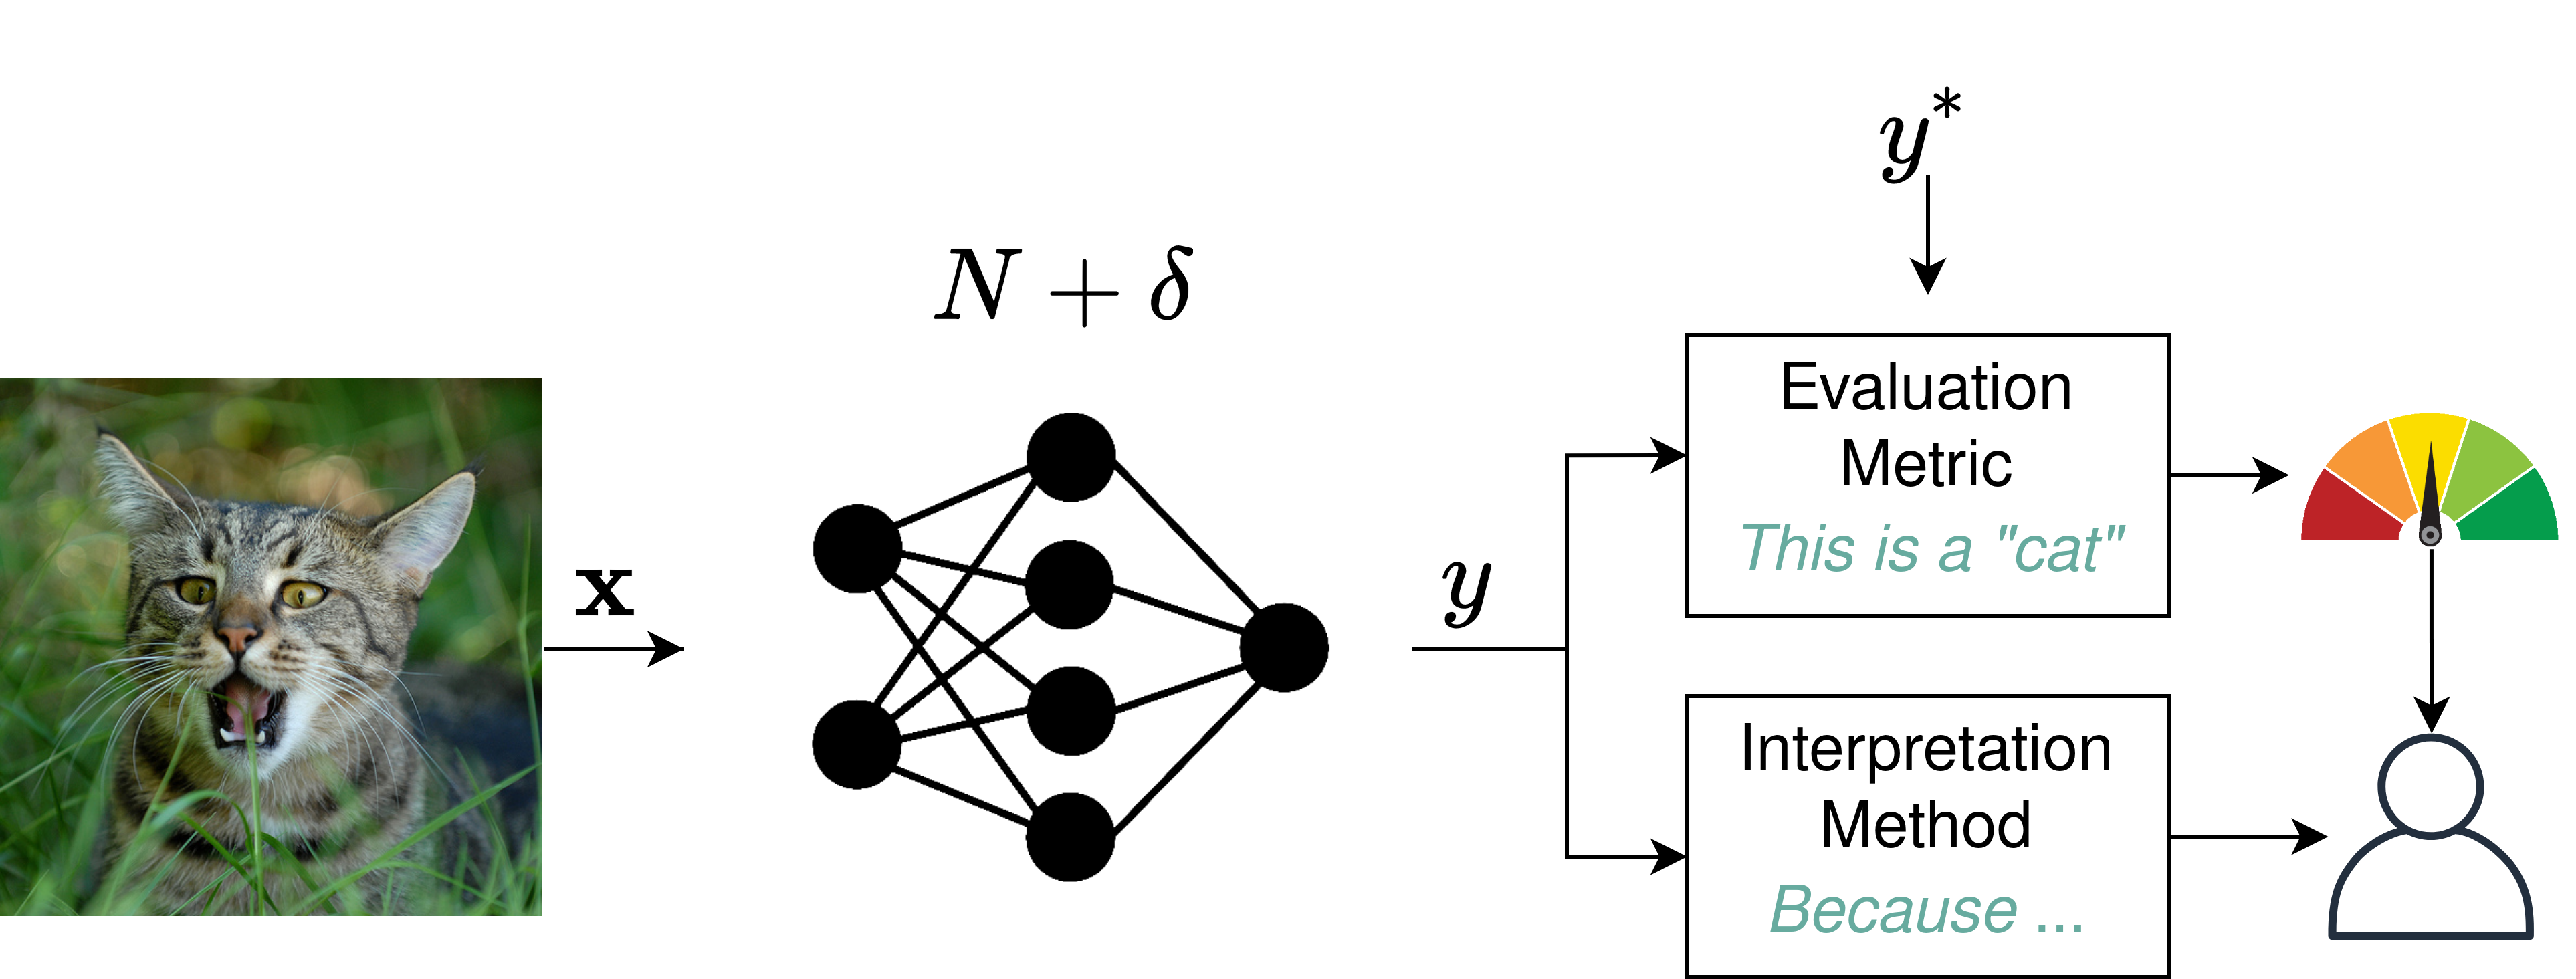
\includegraphics[width=\linewidth]{figures/model_manipulations.png}
    \caption{Depiction of an adversarial model manipulation. The model is fine-tuned with the same distribution of input data and a fooling loss, thus yielding the biased model $N+\delta$.}
    \label{fig:input_manipulation}
    \vspace{-0.3cm}
\end{figure}

%%%%%%%%%%
\subsubsection{Manipulation Targets}
\label{subsubsec:manipulation_targets}

\par\smallskip
\noindent
In addition to the categorization of manipulation methods based on the manipulation level, the methods can further be categorized based on the target of their perturbation. The first possibility is \textit{untargeted} perturbation, the second is \textit{targeted} perturbation. Both these styles can be applied on either model and input level. 

\mypar{Untargeted Manipulations.} 
The majority of manipulations is untargeted, meaning that the applied perturbations are mostly random and not designed to change the prediction for a specific portion of an input sample. 

\mypar{Targeted Manipulations.} 
On the contrary, targeted manipulations aim at specifically changing the explanation of certain features of an input instance \cite{fooling_nn_interpreters}, and sometimes even changing the interpretation of specific classes \cite{simonyan2013deep}. Such a specific feature might be an object in the input image in the context of image classification. \cite{fooling_nn_interpreters} for instance introduce a fooling scheme in which the interpretations of the target classes elephant and school bus are swapped. 
Manipulations on the level of the model are mostly targeted, as the explanation methods are being fooled by adapting the model parameters. 

% Model manipulations pose a much higher threat for deploying the models: If a model itself is changed to explicitly, systemactically fool an explanation method, the bias of the model is internal and much harder to reveal than just a different sort of input into the model. 

%%%%%%%%%%%%%%%%%%%%%%%%% 
\subsection{Evaluation Criteria}
\label{subsec:eval_criteria_manipulations}
Besides the necessary properties of a successful interpretation manipulation method, other evaluation criteria are important to access the success of a fooling method as well as to enable the comparison between different fooling methods. These criteria are informally defined in the following.

\mypar{Effectiveness.} The manipulation scheme is inexpensive to conduct. Input manipulations are by definition inexpensive, as the perturbation can be applied to single input samples. Model manipulations are more expensive as they require tho model parameters to be adapted. However, an adversarial model can be obtained by fine-tuning the model with an adapted objective function. This fine-tuning also has the advantage that the model is adapted to include a systematic bias and can thus be applied to fool explanation methods without further adapting the model or input samples after the fine-tuning step. Furthermore, this systematic bias is hidden in the model, and is hard to uncover. Input manipulations can only fool the model when the inputs are always manipulated. 

\mypar{Transferability.} The manipulation does not only fool one type of interpretation method, but it's effect transfers to other interpretation techniques. 
% This property is naturally given for the class of model manipulations


\mypar{Generalisation.} Generalization of an attack refers to the transfer of fooling to other test samples. This is noteworthy since a manipulation method might only perturb the decision boundary locally around the training points, i.e. only influencing training instances and their neighbors. However, it is desired that the explanations of unseen samples are affected as well. Furthermore, not only unseen samples intarpretations, but also samples that are far away in the feature space should be affected. 
Otherwise, the perturbation is only local around the training points, thus the perturbation does not generalize. 
% On the contrary, model manipulations are non-local perturbations, meaning that they do not merely perturb an input sample
% but rather effect all samples in the way that the model itself is changed. 
% TODO iid ood?
% The  generalisation  of  the  attack  to  testpoints  is  noteworthy  since  we  might  expect  that  the  deci-sion boundary would be perturbed locally around the train-ing points to affect only their explanations, without signifi-cant change for test points, especially if far away in featurespace (see Appendix for more)

\par\smallskip
As outlined in section \autoref{sec:manipulation_methods}, there exists a plethora of interpretation methods differing in the assumption about the model character and also with respect to how interpretations are obtained. Thus, reliable evaluation methods are required allowing for a choice of an appropriate and robust interpretation method. Ultimately, the accordance to these evaluations should naturally allow for choosing an appropriate and robust intarpretation method.  
Evaluations of the quality of an explanation method are separated into qualitative and quantitative evaluations. 

\mypar{Qualitative Evaluation.} 
Inspection and random sampling are commonly used techniques to obtain an intuition about the effect of manipulations. 
As interpretations are attributed to input features, the resulting relevance values $l$ can be easily mapped to the input vector $\mathbf{x}$. Visual inspection of these evaluations for specific samples is informative, but does not allow for general statistics and validation of manipulation effects. Thus, quantitative evaluations are required. 
\cite{adebayo2018sanity} consider two kinds of visualizing saliency maps: 
\begin{itemize}
    \item \textbf{Absolute Value (ABS).} Saliency maps visualized this way show only the absolute values of the normalizem maps.
    \item \textbf{Diverging. } The diverging visualization indicates positive and negative importance in different colors. 
\end{itemize}

\mypar{Quantitative Evaluation.} 
As the goal of interpreter manipulations is to fool an interpreter, thus altering the output of in interpreter, it is straightforward to compare interpretations and data samples before and after perturbation \cite{ghorbani2019interpretation}.

As interpreter manipulations shall alter the output of an interpretation methods while keeping the prediction of a model unchanged, the following metrics 

\begin{itemize}
    \item \textbf{Fooling Success Rate (FSR).} \cite{fooling_nn_interpreters} introduce the concept of the Fooling Success Rate (FSR). The FSR captures the relationship between the model's predictive accuracy and the correctness of the interpretation averaged over multiple test samples. The 'correctness' of the interpretation is the difference between the original interpretation methods output and the output of the same interpretation method when applied to either an adversarial input sample or adversarial model. 
    The FSR counts samples for the model's prediction did not change but for which the interpretation method's output changed as a successfully fooled example. Thus, the higher the FSR, the the more often the fooling is successful in fooling the interpretation method. 
    \item \textbf{Area Over Prediction Curve (AOPC). } AOPC \cite{samek2016evaluating} is a principled way of quantitatively evaluating that the interpretations found by interpretation methods are valid, i.e. based on the features that the model truly uses for making the predicton. \cite{fooling_nn_interpreters} use this measure to ensure that their adversarial model training does not fool the model (i.e. the predictive accuracy of the model is unchanged), but does fool the interpretation method.
\end{itemize}

As the goal of interpreter manipulations is to fool an interpreter, thus altering the output of in interpreter, it is straightforward to compare interpretations and data samples before and after perturbation \cite{ghorbani2019interpretation}.
There are metrics that are applied to identify changes in salient features for any task:
\begin{itemize}
    \item \textbf{Spearman's rank order correlation.} As interpretation methods rank the features based on their importance, the rank correlation \cite{spearman1961proof} is a natural meusure for comparing interpretations. 
    \item \textbf{Intersection of the top-$k$ features.} For some tasks, only the top-$k$ features are relevant, such that a comparison between these top-$k$ features is insightful. 
\end{itemize}

Contrary, the following metrics are used only in computer vision tasks. They have been used in literature to quantify similarities between natural images and remove duplicates. Therefore, they are used in XAI research to compare the changes between saliency maps before and after manipulation for computer vision tasks.
\begin{itemize}
    \item \textbf{Structural Similarity Index (SSIM).} SSIM values are relative similarity measure in the range $\left[0, 1\right]$, where larger values indicate higher similarity.
    \item \textbf{Pearson Correlation Coefficien (PCC).} PCC is also a relative similarity measure returning values in the range $\left[0, 1\right]$. Larger values indicate higher similarity.
    \item \textbf{Pearson Correlation of the Histogram of Gradients\newline (HOG). } Used by \cite{adebayo2018sanity} to indicate the intensity of change between two images. 
    \item \textbf{Mean Squared Error (MSE).} As an absolute error measure, values close to zero indicate high similarity. 
\end{itemize}

\noindent Note that these are only examples without demand for completeness. For further information see \cite{adebayo2018sanity}.
Normalizing these measures to yield values in $\left[0, 1\right]$ with a sum of one is good practice. 
Note that defining similarities that are similar to human vision is still an active area of research. 

%%%%%%%%%%%%%%%%%%%%%%%%%%%%%%%%%%%%%%%%%%%%%%%%%%%%%%%%%%%%%%%%%%%%%%%%%%%%%%%%%%%%%%%%%%%%%%%%%%%%%%%%
%%%%%%%%%%%%%%%%%%%%%%%%%%%%%%%%%%%%%%%%%%%%%%%%%%%%%%%%%%%%%%%%%%%%%%%%%%%%%%%%%%%%%%%%%%%%%%%%%%%%%%%%
% \section{Interpreter Manipulation Method Examples}
\label{sec:manipulations}

After introducing the terminology of model interpreters and manipulation methods in the previous chapters, this chapter gives detailed information about recent manipulation methods. This section also provides insight into major findings in the field of manipulating model interpretations. First, input level manipulations are discussed, followed by model level manipulations. 

\subsection{Input Level Manipulations}

\mypar{Fooling both Model and Interpreter. }\newline
\cite{subramanya2019fooling} design adversarial attacks that fool the machine learning model as well as the model interpretation. 
They design targeted and untargeted input patches superimposed onto original images and then fed into an image classification network and the intperpretation method GradCAM. 

The authors conclude that GradCAM does not reliably highlight the true cause of the prediction decision made by the model. 
Top-1 predicted label 

The authors compare targeted and untargeted patches as well as uniform patches and randomly disturbed ones. 


\mypar{Model-agnostic Interpreters can be gamed.}\newline
%%%%%%%%  %%%%%%%% Fooling LIME and SHAP: Adversarial Attacks on Post hoc Explanation Methods
% https://arxiv.org/pdf/1911.02508.pdf 
\cite{advlime_aies20} propose a framework for fooling the model-agnostic interpreters LIME and SHAP. Their method successfully hides the biases of models trained on adversarial examples by... 
The authors take a statistical approach model-agnostic interpretation methods. They examined the data produced by LIME and SHAP and showed that the perturbed samples are out-of-distrubution samples compared to the distribution of the regular trainging data. 

\autoref{fig:slack_ood_data} shows that the data samples generated by LIME are distributed differently than the data original, non-perturbed data samples. 

\begin{figure}[ht]
    \centering
    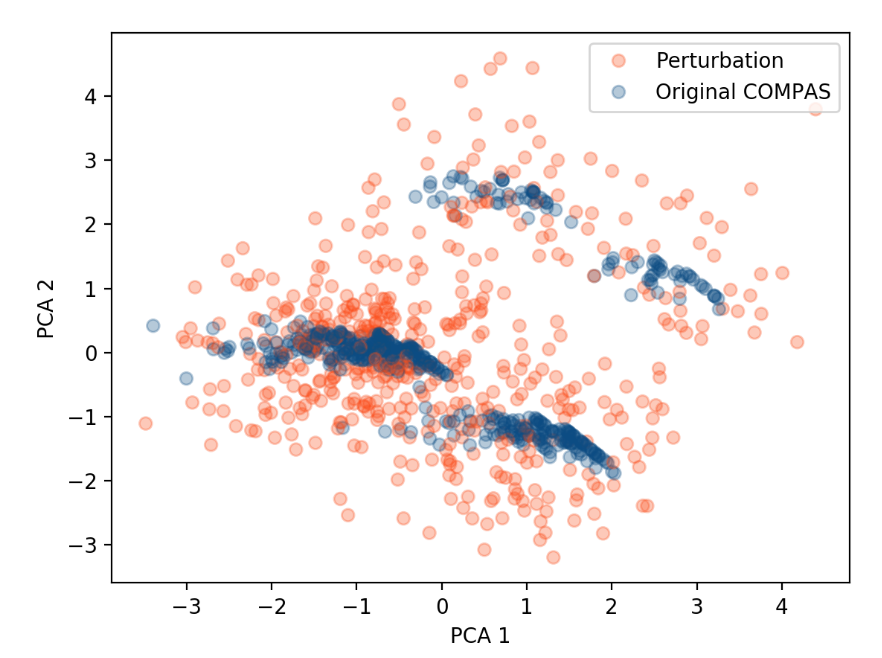
\includegraphics[width=\linewidth]{figures/slack_ood_data.png}
    \caption{Principal Component Analysis (PCA) on the original data (orange) of the COMPAS dataset and the samples perturbed by LIME (blue). Note that the differences are obvious even in the space reduced to two dimensions.}
    \label{fig:slack_ood_data}
    \vspace{-0.3cm}
\end{figure}

\mypar{Saliency Maps are vulnerable to Adversarial Attacks.}
\cite{ghorbani2019interpretation} showed that importance scores produced by the popular interpretation methods Simple Grad, DeepLIFT and TODO. 

\subsection{Model Level Manipulations}
The studies on model manipulation outlined so far have shown that \textit{input perturbations} can make interpretations worse for the same model and interpreter. The articles in this section show that \textit{perturbed model parameters} can also make explanations worse for the same input and interpreter.

\mypar{Adversarial Model Fine-Tuning Fools Multiple Interpreters.}\newline
\cite{fooling_nn_interpreters} were the first to introduce adversarial model manipulations for fooling interpretation methods. The authors adapted the fine-tuning stage of image classification models by using an altered fooling loss function. This loss function is a combination of the standard cross entropy loss function (to maintain the prediction performance) and an additional adversarial term. The adversarial term is used to encourage the interpretation method to give bad interpretations. The results show that the interpretation results are significantly altered while the classification accuracy is maintained. 
This indicates, that the model is robust to the attack, while the interpretation technique is very sensitive. 
Two categories of fooling methods are introduced: 
\begin{itemize}
    \item \textbf{Passive Fooling}, describing the adaption of the adversarial loss term to fool the interpretation method into highlightish uninformative pixels in the input image. Example results from the paper are in \autoref{fig:heo_intro}. The baseline column shows that the interpretation method applied to the original image highlights pixels within the elephant as highly important for the network prediction. After fine-tuning the model with the adversarial loss, the effect of fooling the interpretation method is visible: Other, rather uninformative pixels are highlighted (see labeled columns two to four in the figure). 
    \item \textbf{Active Fooling} is a method with the aim of causing the interpreter to highlight a completely different object in the image, i.e. to make the interpreter actively create false interpretations. This is realized by rewriting the loss function to minimize TODO.
\end{itemize}

\begin{figure}[ht]
    \centering
    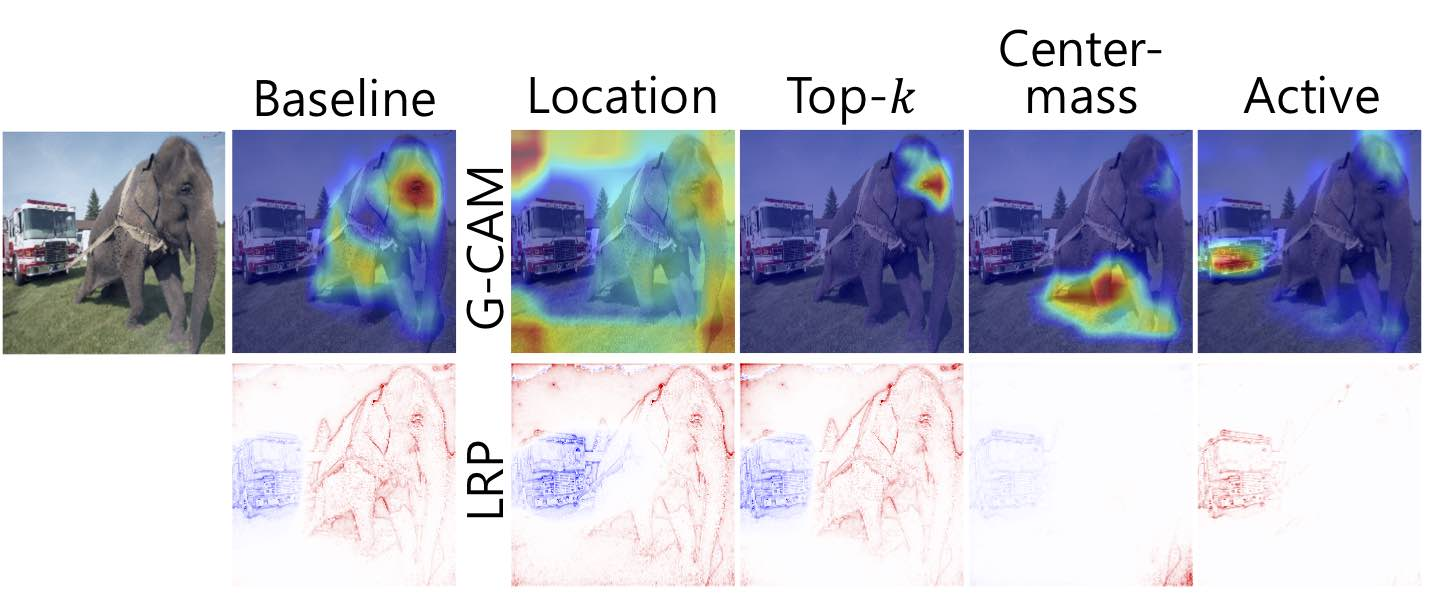
\includegraphics[width=\linewidth]{figures/heo_intro.jpg}
    \caption{}
    \label{fig:heo_intro}
    \vspace{-0.3cm}
\end{figure}

The authors also conduct an analysis to prove that the interpretations are valid. This is done by using the AOPC metric \cite{samek2016evaluating}. 
They find that all interpreters are fooled to a certain degree, and that the foolings furthermore generalize to other interpreters and especially to the whole validation set. It is worth noting that the proposed attack could not easily fool SmoothGrad, indicating that this is a better, or at least more robust interpretation method. 







The authors find that SmoothGrad is less susceptible to model manipulation, while all other interpreters ()

The main point the authors are trying to make is that machine models can be systematically manipulated to contain unfair biases. They prove that such biases can be explicitly encoded into the loss function during the training stage, which yields an adversarial classifier that will generalizes the learned bias to unseen test samples. This is dangerous, as the bias cannot be uncovered unless one has access to the full training pipeline. As interpretation methods claim to uncover the features a model uses for its decision. 


After fine-tuning the model with the regular classification loss combined with an adversarial loss, they investigated if the interpreter results change as a function of model parameters. 
Two types of fooling methods were introduced, namely \textit{active} and \textit{passive} fooling. 

% HEO: The authors find that perturbed model parameters can also make explanations worse for the same input images and interpreters. 
% \subsubsection{Transferability of Manipulations}
% \cite{fooling_nn_interpreters} find that fooling one explanation method with a fooling scheme transfers to other methods. 

%%%%%%%%  %%%%%%%%
\mypar{}
\cite{dimanov2020you} examine the relation of interpretation methods and the concept of fairness. They propose to learn a modified model with concealed unfairness. This is done by fine-tuning a classification model with a loss function extended by an explanation loss. 

Their approach differs methodologically to \cite{fooling_nn_interpreters} as follows: 
\cite{fooling_nn_interpreters} adapt the standard cross entropy loss function by taking the gradient of the correct label ellement from the logits layer, while \cite{dimanov2020you} use the gradient of the cross-entopy loss. 
Taking the gradient of the cross-entropy loss conveys more information about other classes, which may contribute to an improved generalization across different interpretation methods and first of all across different test samples. 

While their approach takes the gradient of the onecorrect label element from the logits layer just before thesoftmax output, we take the gradient of the cross-entropyloss. 

They define adversarial models that focus only on sensitive features which are not informative for the ground truth decision. 


%%%%%%%%%%%%%%
% Conclusions based on the presented studies

\section{Interpreter Manipulation Method Examples}
\label{sec:manipulations}

After introducing the terminology of model interpreters and manipulation methods in the previous chapters, this chapter gives detailed information about recent manipulation methods. This section also provides insight into major findings in the field of manipulating model interpretations. First, input level manipulations are discussed, followed by model level manipulations. 

% TODO \\
% Most of the explanation methods outlined in sec. \autoref{sec:interpretation_methods} have been shown to be vulnerable to adversarial perturbations. 
% Manipulation methods often show that there exist small feature changes resulting in a change of the explanation methods output while the output of the model itself does not change. 
% Most approaches aim at providing a relevance measure of the input features. \\

% Creation of a fooled model by fine-tuning the model with a fooling loss. 
% https://github.com/rmrisforbidden/Fooling_Neural_Network-Interpretations/blob/master/Materials/PPT.pdf 

\subsection{Input Level Manipulations}

\mypar{Fooling both Model and Interpreter. }\newline
\cite{subramanya2019fooling} design adversarial attacks that fool the machine learning model as well as the model interpretation. 
They design targeted and untargeted input patches of various styles, which overlaid onto the original images. 
\autoref{fig:patch_fooling} shows that GradCAM is fooled by this simple method as well as the calssification model, resembling findings in research on adversarial attacks on models. 

\begin{figure}[ht]
    \centering
    \begin{subfigure}{0.32\linewidth}
      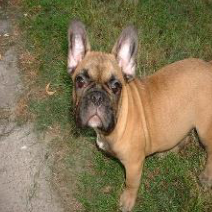
\includegraphics[width=\linewidth]{figures/patch_original.png}
      \caption{\scriptsize{Original. \newline Pred: 'French bulldog'.}}
      \label{fig:patch_original}
    \end{subfigure}
    \begin{subfigure}{0.32\linewidth}
      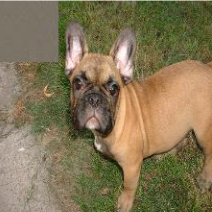
\includegraphics[width=\linewidth]{figures/patch_plus_dog.png}
      \caption{\scriptsize{Original with\newline Patch.}}
      \label{fig:patch_plus_dog}
    \end{subfigure}
    \begin{subfigure}{0.32\linewidth}
      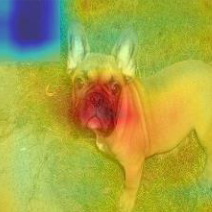
\includegraphics[width=\linewidth]{figures/patch_fooled.png}
      \caption{\scriptsize{Fooled Map, fooled \newline model. Pred: 'Soccer ball'.}}
      \label{fig:patch_fooled}
    \end{subfigure}
    \caption{Fooling of the model and GradCAM. The interpreter is fooled is it takes the original target classe's features as evidence for the wrong class. Images from \cite{subramanya2019fooling}.}\label{fig:patch_fooling}
    \vspace{-0.3cm}
\end{figure}

\mypar{Imperceptible Perturbations significantly alter interpretations. }
\cite{dombrowski2019explanations} show the pendant of adversarial model attacks for interpretation methods: They apply visually imperceptible perturbations to input images, that do not cause the model to misclassify but that cause the interpreter to yield significantly different interpretations. Perturbed images are constructed by using a generative model minimizing the distance to a target map, see \autoref{fig:dombr}. They also propose to make interpretation results better by smoothing the interpretation process, thus providing a way to undo the fooling of the interpreters (e.g. using $\beta$ smoothing).

\begin{figure}[ht]
    \centering
    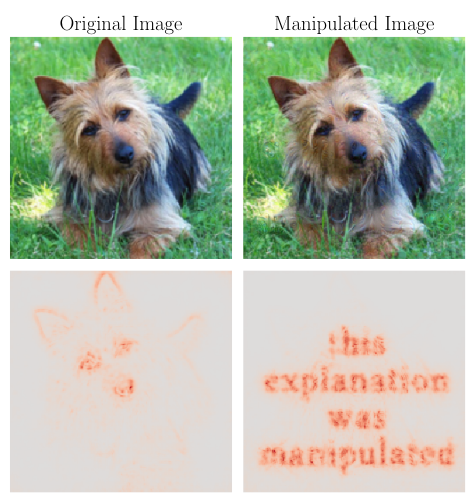
\includegraphics[width=0.8\linewidth]{figures/dombr.png}
    \caption{On the left, the original image with corresponding interpretation map is shown. The right column shows the imperceptibly perturbed input image and it's explanation. The target interpretation map was chosen to be an image with the text "this explanation was manipulated". Image from \cite{dombrowski2019explanations}.}\label{fig:dombr}
    \vspace{-0.3cm}
\end{figure}

\mypar{Saliency Maps are vulnerable to Adversarial Attacks.}
\cite{ghorbani2019interpretation} showed that importance scores produced by the popular the saliency-based interpretation methods SimpleGrad, DeepLIFT and Integrated Gradients are susceptible even to random perturbations. Contrary to \cite{dombrowski2019explanations}, the authors argue that the interpretation methods are actually not broken by these perturbations. They state that saliency-map based approaches are very sensitive, thus reacting to the infinitesimal perturbation of an input $\mathbf{x}$ to $\mathbf{x}+\delta$ with an appropriate change in their output.

\subsection{Model Level Manipulations}
The studies on model manipulation outlined so far have shown that \textit{input perturbations} can make interpretations worse for the same model and interpreter. The articles in this section show that \textit{perturbed model parameters} can also make explanations worse for the same input and interpreter.

\mypar{Adversarial Model Fine-Tuning Fools Multiple Interpreters.}\newline
\cite{fooling_nn_interpreters} were the first to introduce adversarial model manipulations for fooling interpretation methods. The authors adapted the fine-tuning stage of image classification models by using an altered fooling loss function. This loss function is a combination of the standard cross entropy loss function (to maintain the prediction performance) and an additional adversarial term. The adversarial term is used to encourage the interpretation method to give bad interpretations. The results show that the interpretation results are significantly altered while the classification accuracy is maintained. 
This indicates, that the model is robust to the attack, while the interpretation technique is very sensitive. 
Two categories of fooling methods are introduced: 
\begin{itemize}
    \item \textbf{Passive Fooling}, describing the adaption of the adversarial loss term to fool the interpretation method into highlighting uninformative pixels in the input image. They develop three types for this, namely top$-k$, center and location fooling. Example results from the paper are in \autoref{fig:heo_intro}, columns two to four. The baseline column shows that the interpretation method applied to the original image highlights pixels within the elephant as highly important for the network prediction. After fine-tuning the model with the adversarial loss, the effect of fooling the interpretation method is visible: Other, rather uninformative pixels are highlighted (see labeled columns two to four in the figure). 
    \item \textbf{Active Fooling} is a method with the aim of causing the interpreter to highlight a completely different object in the image, i.e. to make the interpreter actively create false interpretations. This is achieved by fine-tuning the model on input images that contain instances from two classes, say the $c_1$=\textit{elephant} and $c_2$=\textit{fire truck} class. The loss with a penalty term that alters the explanations of $c_1$ and $c_2$. The effect of this successful active fooling can be observed in \autoref{fig:heo_intro}, rightmost column.
\end{itemize}

\begin{figure}[ht]
    \centering
    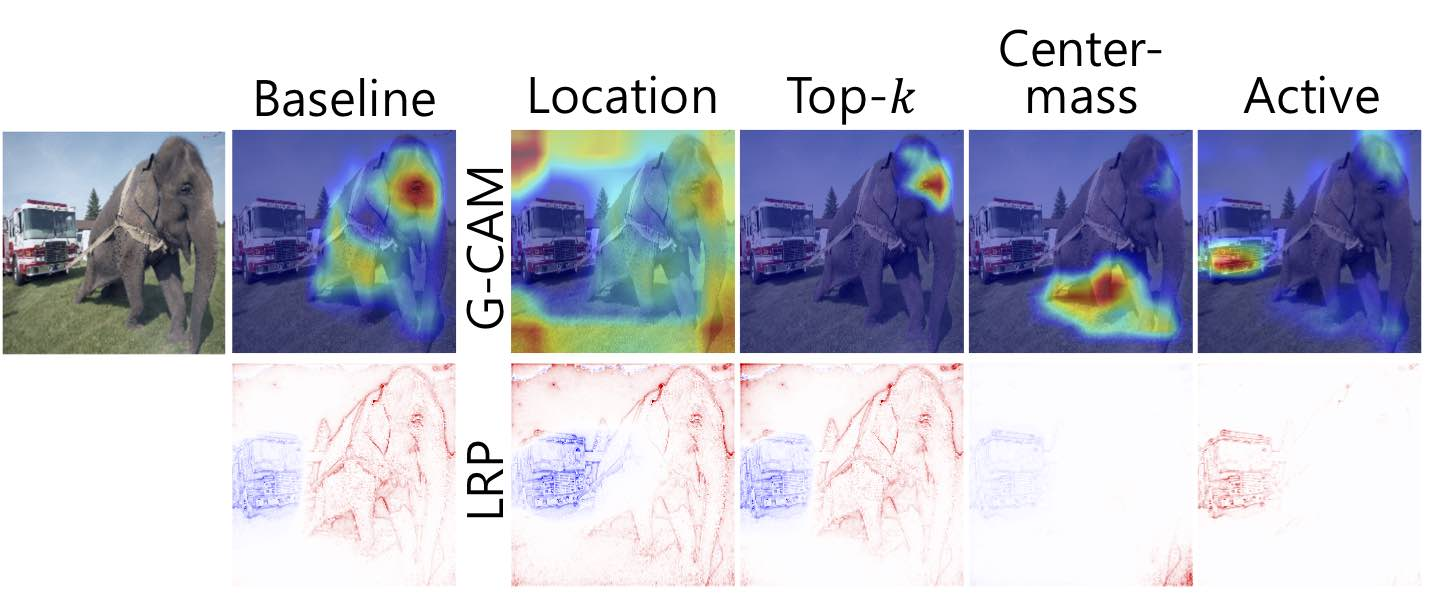
\includegraphics[width=\linewidth]{figures/heo_intro.jpg}
    \caption{Fooling of LRP and GradCAM. Passive fooling causes the interpreters to highlight wrong, uninformative pixels. Active shifts the interpreters indications from a correct class (\textit{elephant}) to a wrong calss \textit{(fire truck}).}
    \label{fig:heo_intro}
    \vspace{-0.3cm}
\end{figure}

% TODO fork it
% The authors also conduct quantitative analysis using the AOPC metric to prove that the interpretations found by the interpreters are valid.
 They find that all tested interpreters are fooled to a certain degree, and that the interpreter malfunctions furthermore generalize to other interpreters and especially to the whole validation set. It is worth noting that the proposed attack could not easily fool SmoothGrad, indicating that this is a better, or at least more robust interpretation method. 

The main point the authors are trying to make is that machine models can be systematically manipulated to contain unfair biases. They prove that such biases can be explicitly encoded into the loss function during the training stage, which yields an adversarial classifier that will generalizes the learned bias to unseen test samples. This is dangerous, as the bias cannot be uncovered unless one has access to the full training pipeline. 

\mypar{Model-agnostic Interpreters can be gamed and model biases can be hidden.} 
%%%%%%%%  %%%%%%%% Fooling LIME and SHAP: Adversarial Attacks on Post hoc Explanation Methods
% https://arxiv.org/pdf/1911.02508.pdf 
\cite{advlime_aies20} propose a framework for fooling the model-agnostic interpreters LIME and SHAP. 
The authors take a statistical approach model-agnostic interpretation methods. They examined the data produced by LIME's and SHAP's perturbation schemes and showed that the perturbed samples are out-of-distribution (o.o.d.) samples compared to the distribution of the regular training data. The authors used this insight, i.e. that LIME and SHAP heavily rely on o.o.d. samples and are thus o.o.d. classifiers, to train an adversarial classifier: This classifier exhibits biased behavior (e.g. using the feature 'race' for predicting the income class of a person) on instances from the original data distribution, while using insensitive features for predicting on o.o.d. samples. It is shown that the interpreters are not able to detect the model bias as they create innocuous interpretations. However, LIME performs slightly better than SHAP. 

This adversarial framework is applied to numerous real-world datasets, and are thus one of the few papers \textit{not} considering computer vision tasks but rather tasks that actually suit the core motivational concern in XAI: That models might be adversarial und unbiased, and that we might not be able to detect that their decision functions are unfair, racist or discriminatory. 
% TODO better explain this

% \autoref{fig:slack_ood_data} shows that the data samples generated by LIME are distributed differently than the data original, non-perturbed data samples. 

% \begin{figure}[ht]
%     \centering
%     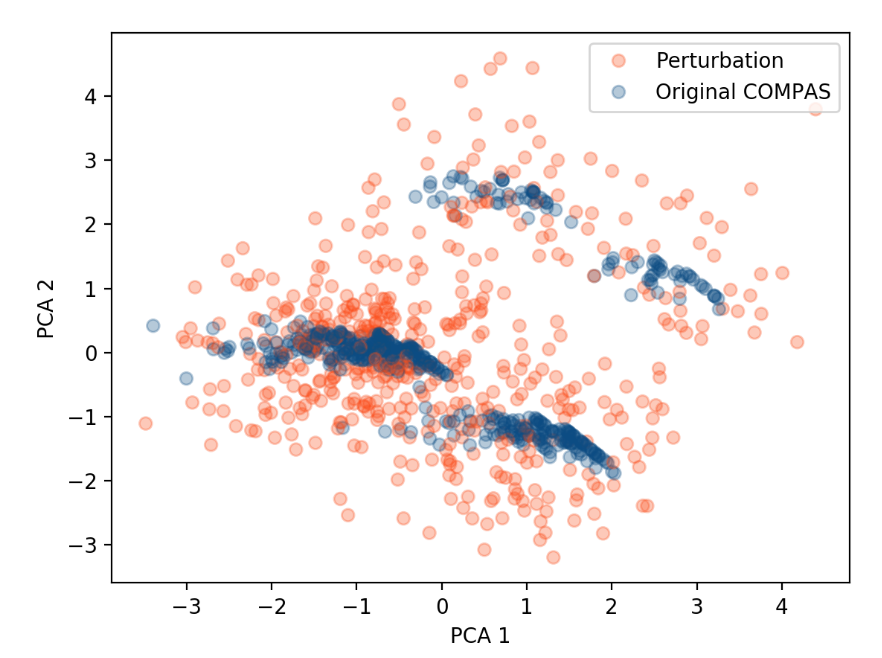
\includegraphics[width=0.8\linewidth]{figures/slack_ood_data.png}
%     \caption{Principal Component Analysis (PCA) on the original data (orange) of the COMPAS dataset and the samples perturbed by LIME (blue). Note that the differences are obvious even in the space reduced to two dimensions.}
%     \label{fig:slack_ood_data}
%     \vspace{-0.3cm}
% \end{figure}

\mypar{Learning Models Which Conceal Unfairness.}
\cite{dimanov2020you} examine the relation of interpretation methods and the concept of fairness. They propose to learn a modified model with concealed unfairness. Their approach differs methodologically to \cite{fooling_nn_interpreters} as follows: 
\cite{fooling_nn_interpreters} adapt the standard cross entropy loss function by taking the gradient of the correct label element from the logits layer, while \cite{dimanov2020you} use the gradient of the cross-entropy loss instead. 
Taking the gradient of the cross-entropy loss conveys more information about other classes, which may contribute to an improved generalization across different interpretation methods and first of all across different test samples. 
Using this method, they are also able to create adversarial models that focus only on sensitive features which are not informative for the ground truth decision. Again, this hidden bias cannot be detected by the examined interpreters. 


%%%%%%%%%%%%%%%%%%%%%%%%%%%%%%%%%%%%%%%%%%%%%%%%%%%%%%%%%%%%%%%%%%%%%%%%%%%%%%%%%%%%%%%%%%%%%%%%%%%%%%%%
%%%%%%%%%%%%%%%%%%%%%%%%%%%%%%%%%%%%%%%%%%%%%%%%%%%%%%%%%%%%%%%%%%%%%%%%%%%%%%%%%%%%%%%%%%%%%%%%%%%%%%%%
% \section{Benchmarking Interpretations}
\label{sec:benchmarking}

Checking the robustness, scope and hence the quality of model interpreters has become an indispensable step in explainable machine learning. 
Evaluating explanation and interpretation methods is difficult as ground truth is mostly lacking. In most applications, it is not known which input features are most important. 

% https://github.com/google-research-datasets/bam 
% https://arxiv.org/abs/1907.09701

\cite{adebayo2018sanity} propose a framework for sanity checking saliency map based interpretation methods. Fer this, a number of randomization tests are introduced along with some visualization techniques and metrics to compare interpretation outputs. The authors find that most methods fail their tests, and warn of the danger of visual assessment. Specifically, they warn that humans tend to chose visually significant appearing images that lack sensitivity to the data distribution and generation as well as to the model. 
However, their findings are so far limited to the domain of computer vision models and tasks. % TODO @outlook
Implementing their randomization tests for other real-world datasets, such as COMPAS \cite{compas_dataset} or the adult income dataset \cite{adult_income} would be an interesting next step. 

Additionally, in order to account for adversarial model manipulations, Heo et al. \cite{fooling_nn_interpreters} propose to expand the criteria for checking the robustness of interpreters further.

\section{Benchmarking Interpretations}
\label{sec:benchmarking}

Checking the robustness, scope and hence the quality of model interpreters has become an indispensable step in explainable machine learning. 
Evaluating explanation and interpretation methods is difficult as ground truth is mostly lacking. In most applications, it is not known which input features are most important. 

% https://github.com/google-research-datasets/bam 
% https://arxiv.org/abs/1907.09701

\cite{adebayo2018sanity} propose a framework for sanity checking saliency map based interpretation methods. Fer this, a number of randomization tests are introduced along with some visualization techniques and metrics to compare interpretation outputs. The authors find that most methods fail their tests, and warn of the danger of visual assessment. Specifically, they warn that humans tend to chose visually significant appearing images that lack sensitivity to the data distribution and generation as well as to the model. 
However, their findings are so far limited to the domain of computer vision models and tasks. % TODO @outlook
Implementing their randomization tests for other real-world datasets, such as COMPAS \cite{compas_dataset} or the adult income dataset \cite{adult_income} would be an interesting next step. 

Additionally, in order to account for adversarial model manipulations, Heo et al. \cite{fooling_nn_interpreters} propose to expand the criteria for checking the robustness of interpreters further.


%%%%%%%%%%%%%%%%%%%%%%%%%%%%%%%%%%%%%%%%%%%%%%%%%%%%%%%%%%%%%%%%%%%%%%%%%%%%%%%%%%%%%%%%%%%%%%%%%%%%%%%%
%%%%%%%%%%%%%%%%%%%%%%%%%%%%%%%%%%%%%%%%%%%%%%%%%%%%%%%%%%%%%%%%%%%%%%%%%%%%%%%%%%%%%%%%%%%%%%%%%%%%%%%%
% \section{Discussion}
\label{sec:discussion}

\footnote{All figures in this article are produced by the author unless noted otherwise.}

% we replicated the findings of the presented manipulation methods from \cite{fooling_nn_interpreters} and.. 

This paper summarizes the current approaches to manipulating model interpretation methods. 
On the one hand, the findings suggest that our models aro not fully aligned with how human information processing works. If machine learning interpretation models would decide by the criteria we humans employ for tasks such as image classification, there would be no fooling of interpretation models by input or model manipulations. 
On the other hand, it was shown that advances in machine learning models has led to models that rely too much on the data they are trained on (the i.i.d. assumption), thus showing a high susceptibility to o.o.d. properties or properties that are highly correlated with labels in the dataset but are not distinctive in the real world (such as image backgrounds). Models and interpreters can still be misled in a large and systematic manner. 

% However, we hope that the vastly expanding and progressing field of XAI will help to move towards more robust, reliable ond human-aligned machine learning models. 

While there exists a number of review papers on XAI and it's various subfields, this report is to the best of our knowledge the first one to comprehensively review manipulation methods for interpreters. 

A growing number of studies gives evidence for model how interpretation methods can be gamed. Among these are the studies outlined in \autoref{sec:manipulations}. Other studies also raise concerns about if standard deep learning practices are valid, such as the work on fooling the broadly used attention mechanism \cite{jain2019attention}. % http://lcfi.ac.uk/media/uploads/files/DimanovBhattJamnikWeller_YouShouldntTrustMe.pdf how  attention-based  methods  could  be  fooled.  (Jainand  Wallace  2019)  showed  that  ‘attention  is  not  explana-tion’, demonstrating that attention maps could be manipu-lated after training without altering predictions

We believe that identifying risks and adversaries helps to open up research on more robust interpretation methods. 

% Interpretation methods can be categorized based on if they maintain local consistency among explanations (i.e. finding an explanation that is true for single data samples and their neighbors) or based on if they try to find global explanations, being true for all samples of a class. 
% As there exist model manipulations methods, that structurally alter the models by adapting tre loss function, this line of global model fooling though being approached is still in its infancy. 


\subsection{Conclusion}

% We believe our algorithms can facilitate developingmore robust network interpretation tools that truly explainthe network’s underlying decision making process. https://openaccess.thecvf.com/content_ICCV_2019/papers/Subramanya_Fooling_Network_Interpretation_in_Image_Classification_ICCV_2019_paper.pdf 
% --> making nns more robust to adversarial attacks might also benefit the robustness of fooling methods?

Finally, it must be noted that the suitability of a method depends on its application domain. 


Much critique has been applied to methods aiming at interpreting complex and potentially non-interpretable models in the domain of computer vision. Some researchers argue it is not worthwhile to study non interpretable systems while dismissing that using inherently interpretable models in the first place might be the better approach. 

Adversarial attacks show that machine learning systems are still fundamentally fragile: They may be successful in a number of tasks, but fail to adapt to o.o.d. scenarios, i.e. when being applied to unfamiliar territory. 
% Our results raise concerns on how interpretations of neural networks can be manipulated.
% fail unpredictably

 The findings about manipulating interpretations do not suggest that interpretations are completely meaningless, just as adversarial attacks on predictions models do not imply that machine learning models are useless. However, they suggest that there still are fundamental flaws in the way neural networks operate und that much caution and supervision sould be applied if they are to be deployed in the real world. 

This paper follows the footsteps of \cite{lipton2018mythos}, trying to caution against blindly putting faith into post-hoc explanation methods. Moreover, we propose that checking the robustness of interpretation methods not only with respect to adversarial input manipulations but also with respect to adversarial model manipulation should be a necessary proof of concept. 


% We argue checking the robustness of interpretation methods with respect to our adversarialmodel manipulation should be an indispensable criterion for the interpreters in addition to the sanitychecks proposed in [27];


%%%%%%%%%%%%% FUTURE WORK
\subsection{Future Work}
We see several possible future directions of future work. 
Firstly, for approaching the discrepency of in-lab and real-life applications of, more focus might be laid in the development better performance metrics for both measuring the performance of machine learning models as well as their interpreters. 
More specifically, it might be fruitful to further investigate the correlation between ood samples and the performance of an interpretation method. So far, most of these findings are limited to specific experimental settings. 


There is also no work proposing a benchmarking for ... 

What is currently sparse is the comparison between different interpretation techniques and the relation of interpretation fragility to the model class, interpretation method and the task type and dataset structure. 


The output of the interpretation method is projected onto the original image for better human readability
--> dangerous to trust this


% % Visually appealing methods and easiy visual assessment of results. 
% Most works in the field of XAI focus on image classification tasks, mostly because visualizations of a neural networks prediction can be easily verified by a human. The general purpose of image classification is to detect what objects are in an image. If a model works can be checked rather easily (if an image contains a cat, the prediction of a neural network should be cat and not some other object category). However, how it works (\textit{interpretability}), i.e. based on which features in the image the decision is made or which parameters in the model influence the prediction most, is an entirely different matter (\textit{explainability}).  

% More importantly, while a big motivation for the development of robust and explainable systems is to overcome biases in models, datasets with direct implication of biases are seldomly used and by far not treated as benchmarking scenarios for explainability analyses.  
\section{Conclusion}
\label{sec:discussion}
% bias detection 

This paper summarizes the current approaches to manipulating model interpretation methods. 
The main insights from literature outlined in \autoref{sec:manipulations} are the following: 
\begin{itemize} % TODO cite papers
    \item Saliency-map based interpreters can be tricked even by simple perturbation methods, such is input patches, which also succeed in fooling models. \cite{subramanya2019fooling}
    \item State-of-the-art interpreters may not be able to detect biases in biased and adversarial models.\cite{dimanov2020you, advlime_aies20}
    \item Biases can be encoded into the model by adapting the loss function and by inexpensively fine-tuning the model. These adaptations can trick the interpretation methods into yielding wrong results while models remain accurate. \cite{fooling_nn_interpreters}
    \item \cite{dombrowski2019explanations} show the pendant of adversarial model  attacks for interpretation methods: They apply visually imperceptible perturbations to input images, that do not cause the models to misclassify but that cause the interpreter to yield significantly different interpretations.
    % \item Two very similar inputs with equal model predictions can be interpreted totally different
\end{itemize}
% Unlike \cite{fooling_nn_interpreters}, \cite{advlime_aies20} take the threat seriously and show on real-world datasets that state-of-the-art interpreters may not aid in detecting severe biases in models. 
On the one hand, the findings suggest that our models aro not fully aligned with how human information processing works. If machine learning interpretation models would decide by the criteria we humans employ for tasks such as image classification, there would be no fooling of interpretation models by input or model manipulations. 
On the other hand, it was shown that advances in machine learning models has led to models that rely too much on the data they are trained on (the i.i.d. assumption), thus showing a high susceptibility to o.o.d. properties or properties that are highly correlated with labels in the dataset but are not distinctive in the real world (such as image backgrounds) in the first place. Models and interpreters can still be misled in a large and systematic manner. 

A growing number of studies gives evidence for model how interpretation methods can be gamed. Among these are the studies outlined in \autoref{sec:manipulations}. Other studies also raise concerns about if standard deep learning practices are valid, such as the work on fooling the broadly used attention mechanism \cite{jain2019attention}.
However, findings about manipulating interpretations do not suggest that interpretations are completely meaningless, just as adversarial attacks on predictions models do not imply that machine learning models are useless. Nonetheless, they suggest that there still are fundamental flaws in the way neural networks operate und that much caution and supervision should be applied when deploying them in the real world. 
This paper follows the footsteps of \cite{lipton2018mythos}, trying to caution against blindly putting faith into post-hoc explanation methods. Moreover, we propose that checking the robustness of interpretation methods not only with respect to adversarial input manipulations but also with respect to adversarial model manipulation should be a necessary proof of concept. 

% However, we hope that the vastly expanding and progressing field of XAI will help to move towards more robust, reliable ond human-aligned machine learning models. 

While there exists a number of review papers on XAI and it's various subfields, this report is to the best of our knowledge the first one to comprehensively review manipulation methods for interpreters. 
We believe that identifying risks and adversaries helps to open up research on more robust interpretation methods. 

 % http://lcfi.ac.uk/media/uploads/files/DimanovBhattJamnikWeller_YouShouldntTrustMe.pdf how  attention-based  methods  could  be  fooled.  (Jainand  Wallace  2019)  showed  that  ‘attention  is  not  explana-tion’, demonstrating that attention maps could be manipu-lated after training without altering predictions


% Interpretation methods can be categorized based on if they maintain local consistency among explanations (i.e. finding an explanation that is true for single data samples and their neighbors) or based on if they try to find global explanations, being true for all samples of a class. 
% As there exist model manipulations methods, that structurally alter the models by adapting tre loss function, this line of global model fooling though being approached is still in its infancy. 


% \subsection{Conclusion}

% We believe our algorithms can facilitate developingmore robust network interpretation tools that truly explainthe network’s underlying decision making process. https://openaccess.thecvf.com/content_ICCV_2019/papers/Subramanya_Fooling_Network_Interpretation_in_Image_Classification_ICCV_2019_paper.pdf 
% --> making nns more robust to adversarial attacks might also benefit the robustness of fooling methods?

% Finally, it must be noted that the suitability of a method depends on its application domain. 


% Much critique has been applied to methods aiming at interpreting complex and potentially non-interpretable models in the domain of computer vision. Some researchers argue it is not worthwhile to study non interpretable systems while dismissing that using inherently interpretable models in the first place might be the better approach. 

% Adversarial attacks show that machine learning systems are still fundamentally fragile: They may be successful in a number of tasks, but fail to adapt to o.o.d. scenarios, i.e. when being applied to unfamiliar territory. 
% Our results raise concerns on how interpretations of neural networks can be manipulated.
% fail unpredictably


% We argue checking the robustness of interpretation methods with respect to our adversarialmodel manipulation should be an indispensable criterion for the interpreters in addition to the sanitychecks proposed in [27];


%%%%%%%%%%%%% FUTURE WORK
\mypar{Future Work.} \newline
We see several possible future directions of future work. Firstly, for approaching the discrepancy of in-lab and real-life applications of machine learning, more focus ought to be laid on the development of better performance metrics for both measuring the performance of machine learning models as well as their interpreters. 
More specifically, it might be fruitful to further investigate the correlation between o.o.d. samples and the performance of an interpretation method. So far, most of these findings are limited to specific experimental settings (e.g. most research on interpretability is focused on computer vision tasks).
Further research should much more explore real world datasets and tasks. The relationship between different interpretation techniques and the dependence of interpretation susceptibility on model class, interpretation method, and task type and dataset structure should also be thoroughly investigated. 


% There is also no work proposing a benchmarking for ... 


% The output of the interpretation method is projected onto the original image for better human readability
% --> dangerous to trust this


% % Visually appealing methods and easiy visual assessment of results. 
% Most works in the field of XAI focus on image classification tasks, mostly because visualizations of a neural networks prediction can be easily verified by a human. The general purpose of image classification is to detect what objects are in an image. If a model works can be checked rather easily (if an image contains a cat, the prediction of a neural network should be cat and not some other object category). However, how it works (\textit{interpretability}), i.e. based on which features in the image the decision is made or which parameters in the model influence the prediction most, is an entirely different matter (\textit{explainability}).  

% More importantly, while a big motivation for the development of robust and explainable systems is to overcome biases in models, datasets with direct implication of biases are seldomly used and by far not treated as benchmarking scenarios for explainability analyses.  


% \cite{fooling_nn_interpreters} propose to measure the quality of an explanation method by their stability with respect to adversarial model manipulations. 

% \balance
\bibliography{mybib}{}
% \bibliographystyle{plain}
\bibliographystyle{ACM-Reference-Format}

\end{document}
\endinput